% Template:     Informe LaTeX
% Documento:    Archivo de ejemplo
% Versión:      7.0.0 (23/06/2020)
% Codificación: UTF-8
%
% Autor: Pablo Pizarro R.
%        Facultad de Ciencias Físicas y Matemáticas
%        Universidad de Chile
%        pablo@ppizarror.com
%
% Manual template: [https://latex.ppizarror.com/informe]
% Licencia MIT:    [https://opensource.org/licenses/MIT]

% ------------------------------------------------------------------------------
% NUEVA SECCIÓN
% ------------------------------------------------------------------------------
% Las secciones se inician con \section, si se quiere una sección sin número se
% pueden usar las funciones \sectionanum (sección sin número) o la función
% \sectionanumnoi para crear el mismo título sin numerar y sin aparecer en el índice

\newcommand{\explorelite}{\textit{explore\_lite}}
\newcommand{\movebase}{\textit{move\_base}}



\section{Pregunta 1}

\subsection{Parte a.-}

Se utilizó una variación porcentual máxima de 0.5\% en todas las unidades generadoras, considerando además la potencia activa máxima de 3kW. Usando la expresión \ref{calculo-mp}, se obtuvo un valor de pendiente droop $M_p = -0.0007$. 

\begin{equation}
    M_p = -\frac{\Delta V}{P_{max}}
    \label{calculo-mp}
\end{equation}

Se obtiene la Figura \ref{conexion-desconexion-potencia-dgs}, donde se observa la potencia entregada por cada unidad de generación, junto a las señales de conexión/desconexión de cargas.

\begin{figure}
    \centering
    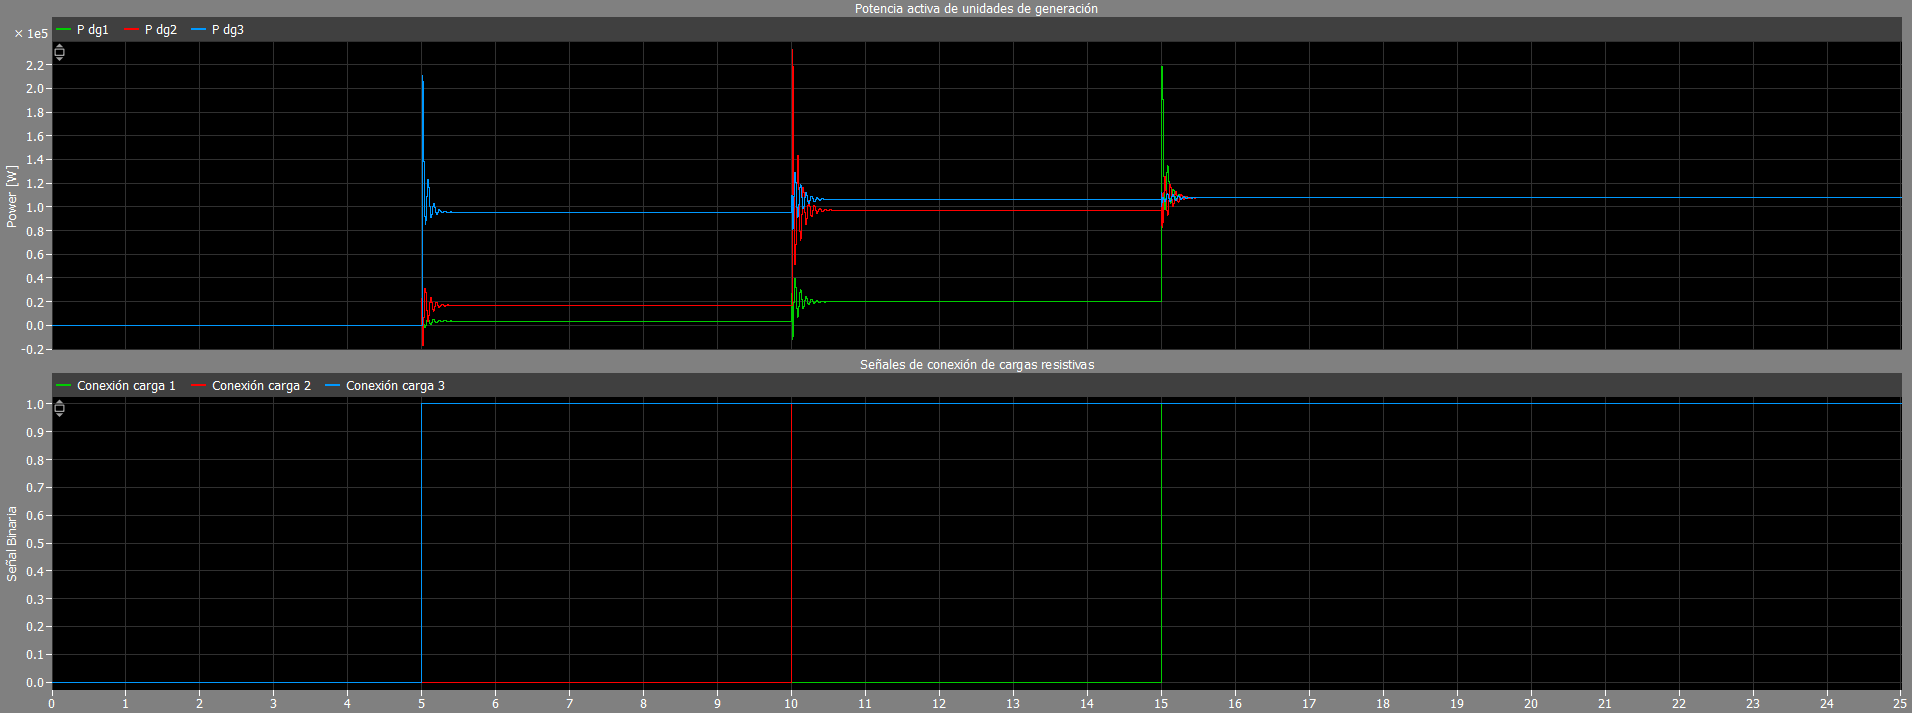
\includegraphics[width=1.0\linewidth]{Tarea 2/report/imagenes/p1a/conexion-desconexion-potencia-dgs.png}
    \caption{Gráfico de potencia entregada por cada unidad de generación, junto a las señales de conexión/desconexión de cargas para una pendiente droop de -0.0007 en cada unidad generadora.}
    \label{conexion-desconexion-potencia-dgs}
\end{figure}

En la parte superior del gráfico, que muestra la potencia activa de las unidades generadoras, se observa que a medida que las cargas se conectan secuencialmente (como se indica en la parte inferior del gráfico con las señales de conexión), la potencia entregada por cada unidad de generación (DG$_1$, DG$_2$, DG$_3$) aumenta de manera coordinada. Este comportamiento es esperado, ya que el control droop permite que la demanda de potencia adicional, debido a las cargas conectadas, se distribuya proporcionalmente entre las unidades generadoras.\\

Se puede ver que DG$_1$ (en verde) es la primera en reaccionar ante la conexión de la primera carga, seguida de DG$_2$ (en rojo) y DG$_3$ (en azul), lo que muestra un aumento en la potencia entregada por cada una de ellas. A medida que se conectan las tres cargas, la potencia aumenta de manera escalonada, reflejando cómo el sistema responde ante la demanda creciente.\\

Dado que las pendientes droop son iguales para las tres unidades generadoras, la potencia se distribuye equitativamente entre ellas, lo que se refleja en la similitud de los picos de potencia generada por DG$_1$, DG$_2$ y DG$_3$ a medida que se conectan las cargas.

\subsection{Parte b.-}

Para esta parte se modificaron las pendientes droop de cada unidad de generación, estableciendo valores diferentes para cada una de ellas. Esta variación en las pendientes permite analizar cómo se redistribuye la potencia entre las unidades generadoras y qué implicancias tiene para la estabilidad y eficiencia de la micro-red.\\

De este modo, se seteó una variación de tensión de 0.5 para la primera unidad generadora, de 1 para la segunda unidad generadora y de 2 parta la tercera y última unidad generadora, obteniendo una pendiente droop de -0.0007 para el DG$_1$, -0.0013 para el DG$_2$ y -0.0023 para el DG$_3$. A continuación se pueden observar los resultados:

\begin{figure}
    \centering
    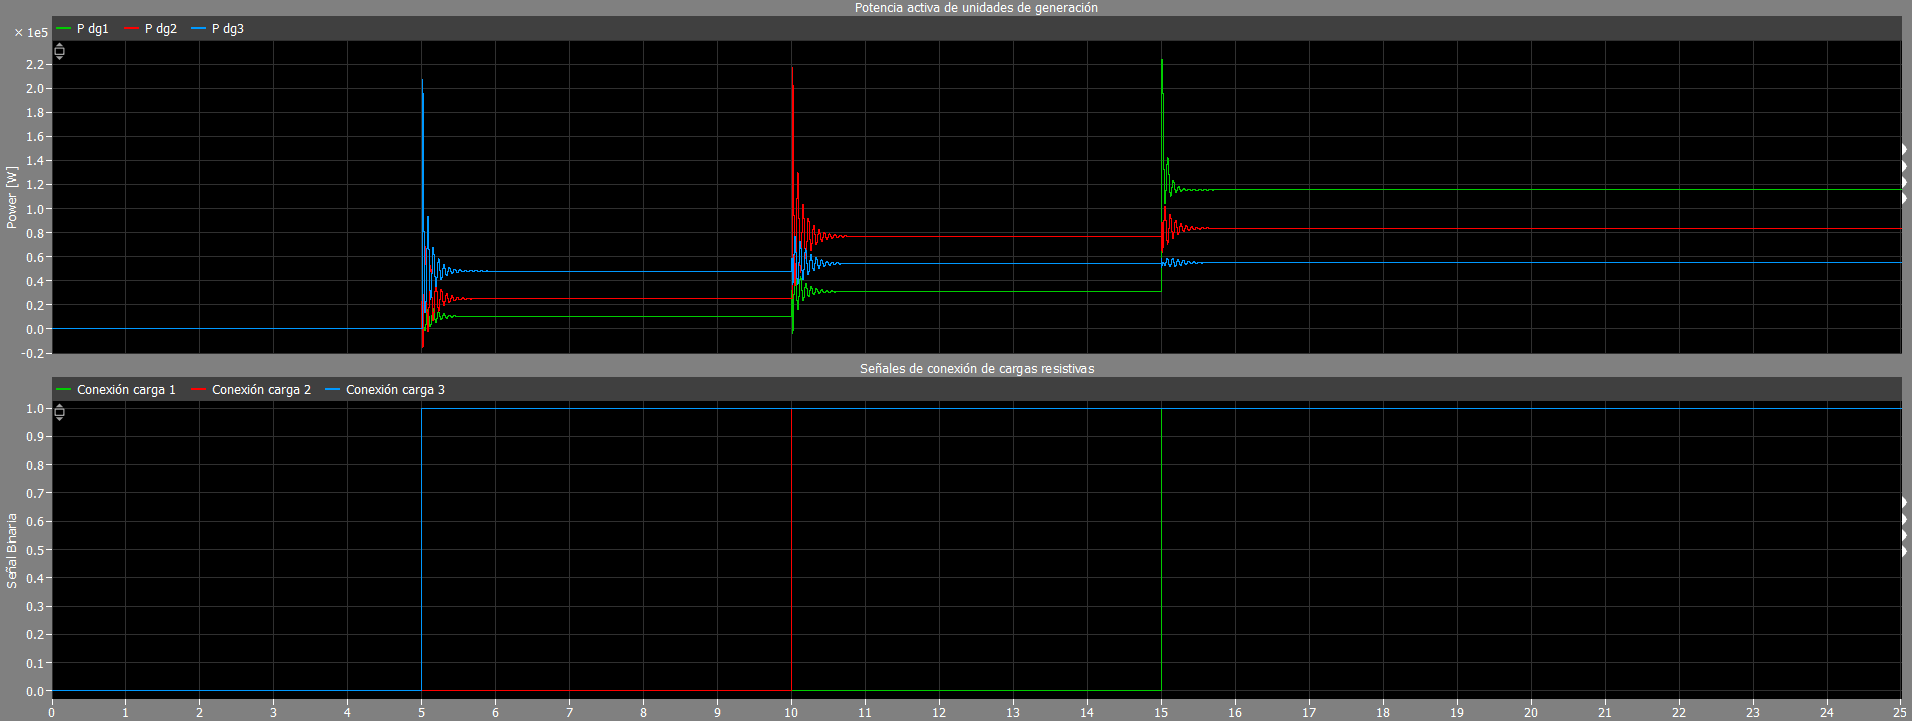
\includegraphics[width=1.0\linewidth]{Tarea 2/report/imagenes/p1b/mp_dist_ok.png}
    \caption{Gráfico de potencia entregada por cada unidad de generación, junto a las señales de conexión/desconexión de cargas para una pendiente droop de -0.0007 para el DG$_1$, -0.0013 para el DG$_2$ y -0.0023 para el DG$_3$.}
    \label{mp_dist_ok}
\end{figure}

Los resultados muestran que, al conectar las cargas, la potencia se distribuye de manera más equilibrada entre las tres unidades. La unidad con la pendiente más baja (DG$_1$) responde generando una mayor cantidad de potencia, mientras que DG$_2$ y DG$_3$, con pendientes más altas, generan proporcionalmente menos potencia. Esto es un comportamiento esperado, ya que las unidades con pendientes más pequeñas son más sensibles a los cambios de carga y, por lo tanto, asumen una mayor parte de la generación de potencia.\\

Este ajuste de pendientes proporciona una respuesta estable del sistema, en la que las tres unidades operan de manera conjunta para suplir la demanda, con DG$_1$ liderando la generación y DG$_3$ proporcionando menos potencia debido a su pendiente mayor. No se observan oscilaciones significativas en la potencia generada, lo que indica que el sistema está bien balanceado. Sin embargo, al seguir subiendo los valores de variación de tensión, el sistema empieza a variar bastante más. Posteriormente, se realizó una simulación seteando una variación de tensión de 0.5 para la primera unidad generadora, de 2 para la segunda unidad generadora y de 4 parta la tercera y última unidad generadora obteniendo una pendiente droop de -0.0007 para el DG$_1$, -0.0033 para el DG$_2$ y -0.0053 para el DG$_3$.

\begin{figure}
    \centering
    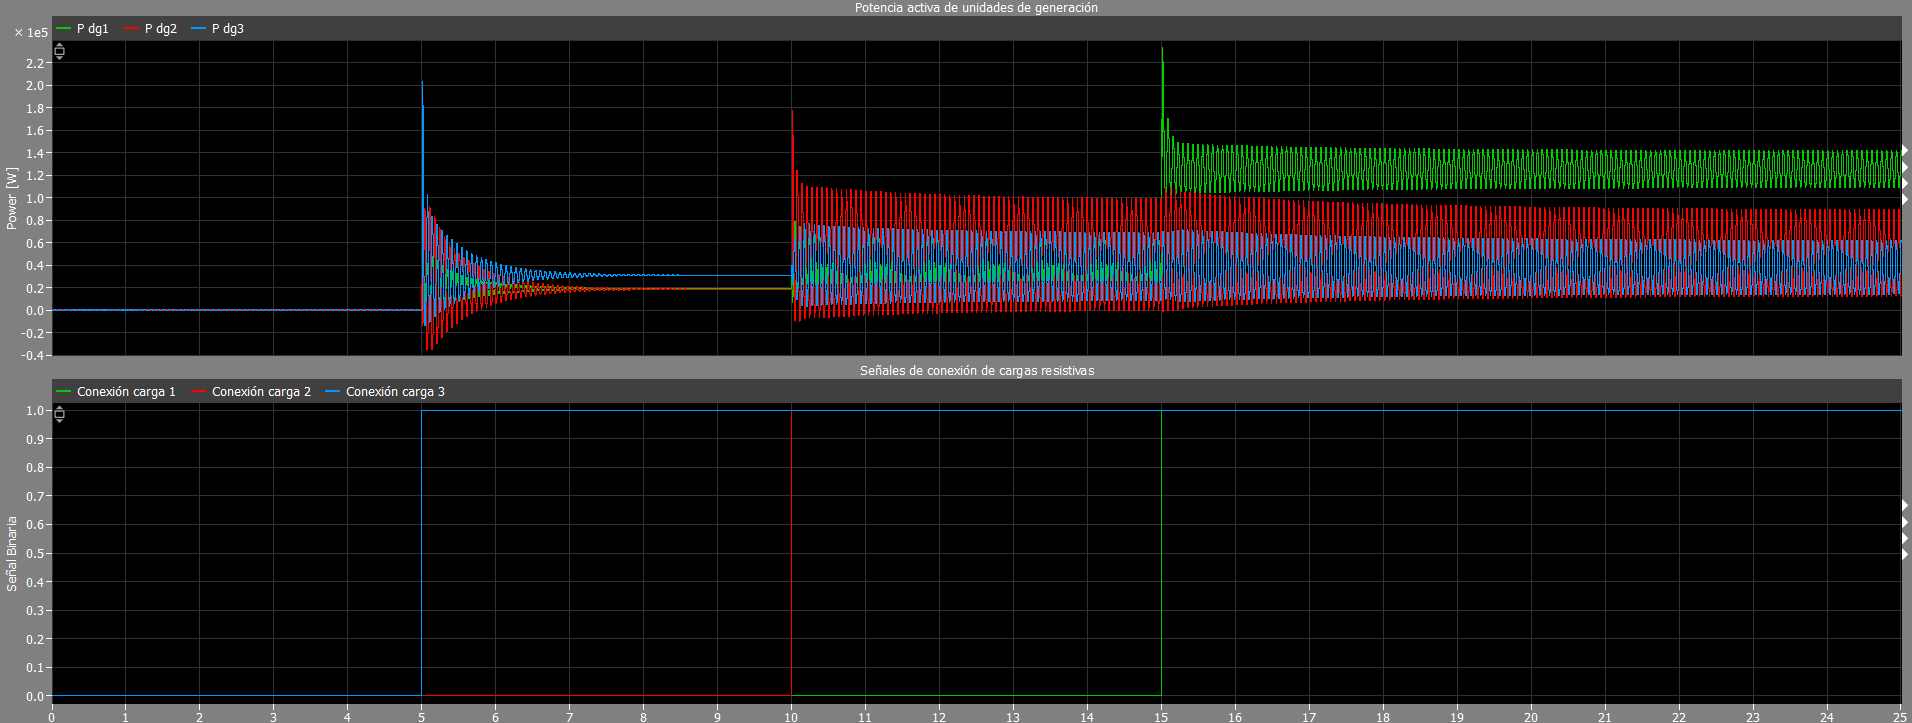
\includegraphics[width=1.0\linewidth]{Tarea 2/report/imagenes/p1b/mp_dist_mal.png}
    \caption{Gráfico de potencia entregada por cada unidad de generación, junto a las señales de conexión/desconexión de cargas para una pendiente droop de -0.0007 para el DG$_1$, -0.0033 para el DG$_2$ y -0.0053 para el DG$_3$.}
    \label{mp_dist_mal}
\end{figure}

Al observar los resultados, se puede notar que este cambio genera una distribución de potencia mucho más desigual entre las unidades. DG$_1$ continúa asumiendo la mayor parte de la generación, mientras que DG$_2$ y, especialmente, DG$_3$ generan muy poca potencia.\\

A medida que las pendientes droop aumentan, las unidades con pendientes más altas se vuelven menos sensibles a los cambios en la demanda de potencia, lo que reduce su contribución a la generación. Este comportamiento puede provocar una carga desproporcionada sobre la unidad DG$_1$, lo que genera oscilaciones más grandes en la potencia total generada, como se observa en la Figura \ref{mp_dist_mal}, donde las oscilaciones se amplifican a lo largo del tiempo. Este fenómeno ocurre porque las unidades con pendientes más altas no responden adecuadamente a las variaciones de carga, dejando que las unidades con pendientes más bajas absorban la mayoría de la demanda.

\section{Pregunta 2}

\subsection{Parte a.-}

Para el diseño del control secundario distribuido DAPI, se implementó un controlador integral que restaura los niveles de tensión en la micro-red. En base a la ecuación \ref{controlador_dapi_tension}, se puede establecer una frecuencia natural dependiente del parámetro $\zeta_1$ de cada unidad generadora. Se establece entonces $\zeta_i = 2\pi f_{i}$. Al tratarse de un control secundario, se busca que su frecuencia natural sea 10 veces más pequeña que la del control primario, para garantizar el desacople de estos. Se decidió usar $\zeta = 2\pi 0.1 = 0.628$ para todas las unidades generadoras en base a la respuesta observada en la Figura \ref{accion_dapi_ok}. \\

Además, de acuerdo a lo visto en cátedra, se definió un tiempo de muestreo de 1 segundo, correspondiente al rango de frecuencia deseado de un control secundario de voltaje.

\begin{equation}
    \zeta_i \frac{dv_i}{dt} = -\gamma_i \left( V_i - V^* \right) - \sum_{j=1}^{n} c_{ij} \left( \frac{P_i}{P_i^*} - \frac{P_j}{P_j^*} \right)
    \label{controlador_dapi_tension}
\end{equation}

A continuación, se presentan los componentes y características del diseño del controlador DAPI:

\begin{figure}
    \centering
    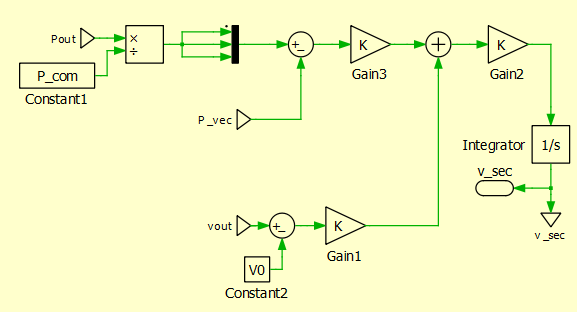
\includegraphics[width=1.0\linewidth]{Tarea 2/report/imagenes/p2a/estructura_dapi.png}
    \caption{Estructura del controlador DAPI.}
    \label{estructura_dapi}
\end{figure}

El controlador DAPI mostrado en la imagen tiene una estructura compuesta por varios bloques que realizan la restauración de la tensión.

\begin{itemize}
    \item P$_{com}$ y P$_{vec}$: Se observa un bloque que toma la señal de referencia de potencia (P$_{com}$) y la compara con la potencia real (P$_{out}$) para generar una señal de error. Esta señal es normalizada utilizando un bloque divisor.
    \item Ganancias y Sumadores: A partir de la señal de error, se utilizan varios bloques de ganancia (denotados como Gain1, Gain2, y Gain3) que ajustan las señales y sumadores que permiten el procesamiento de las variables de control.
    \item Integrador: El bloque integrador es el encargado de realizar la acción integral del controlador, lo que permite corregir cualquier error acumulado en el sistema y restaurar la tensión a su valor de referencia (v$_{sec}$).
    \item V0 y v$_{out}$: La diferencia de la tensión medida con la referencia de tensión (v$_{out}$) también es procesada y ajustada por una constante para que el controlador realice la corrección de manera adecuada.
\end{itemize}

Como se mencionó anteriormente, se buscó que la frecuencia del DAPI fuera 10 veces más pequeña que la del control droop, por lo que para las simulaciones se seteó una frecuencia de control droop (desacople) de 2 Hz, mientras que la frecuencia del DAPI se estableció en 0.1 Hz. A continuación, se muestran los voltajes obtenidos a partir de la acción de consenso junto a las señales binarias que indican las conexiones de las cargas:

\begin{figure}
    \centering
    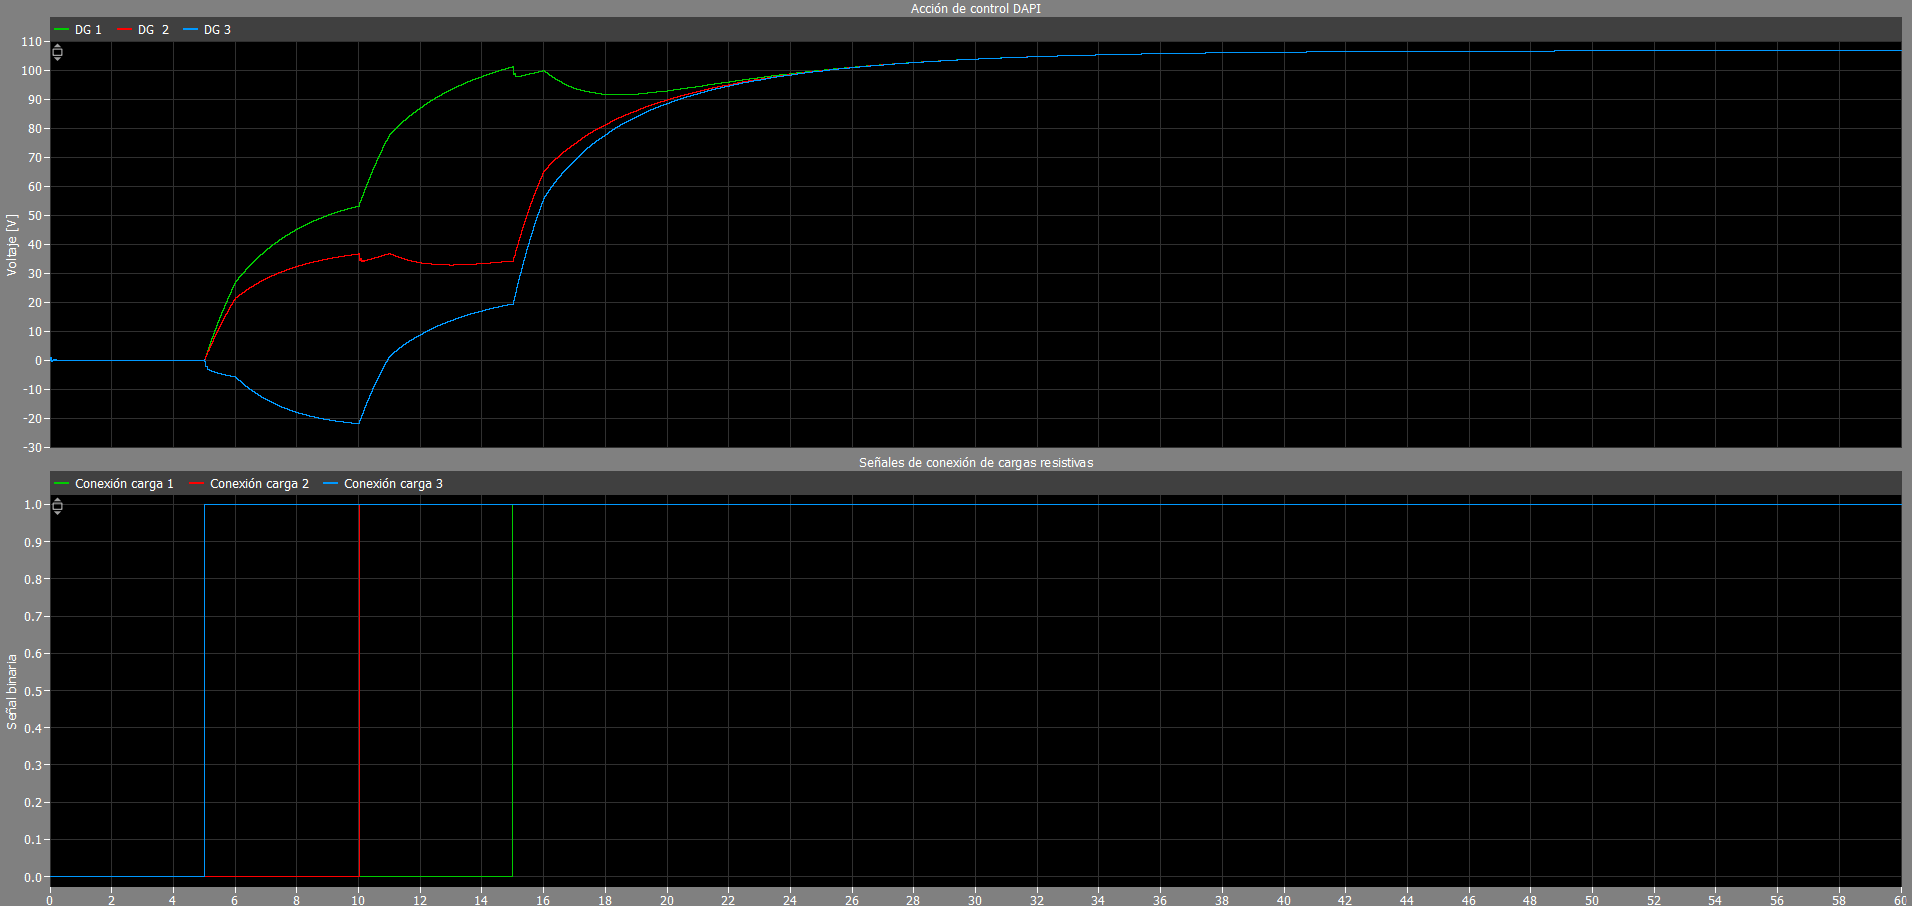
\includegraphics[width=1.0\linewidth]{Tarea 2/report/imagenes/p2a/accion_dapi_ok.png}
    \caption{Gráfico de voltajes de cada unidad de generación, junto a las señales de conexión/desconexión de cargas para una frecuencia de desacople de 2 Hz y una frecuencia del DAPI de 0.1 Hz.}
    \label{accion_dapi_ok}
\end{figure}

En un primer instante, los voltajes de las tres unidades comienzan en valores cercanos a cero, ya que no hay demanda de potencia significativa. A medida que las cargas se conectan progresivamente (señales en la parte inferior del gráfico), se aprecia una respuesta inmediata en los voltajes de las unidades generadoras. La acción del controlador DAPI es visible en la forma en que los voltajes de cada unidad se ajustan de manera gradual hacia sus valores de referencia. De forma separada, las acciones de cada unidad son:
\begin{itemize}
    \item DG$_1$ (verde): Esta unidad muestra la respuesta más rápida, alcanzando el valor de referencia antes que las demás. Esto puede deberse a una mayor capacidad de ajuste del controlador para esta unidad, lo que asegura que asuma una mayor parte de la carga inicial de la micro-red.
    \item DG$_2$ (rojo): La segunda unidad, aunque también responde a la conexión de la carga, lo hace de manera más lenta y con un comportamiento más estable después de las primeras oscilaciones.
    \item DG$_3$ (azul): La última unidad muestra una respuesta más lenta que las anteriores, ajustando su voltaje de manera progresiva para alcanzar su referencia en los últimos instantes de la simulación.
\end{itemize}

En cuanto a la acción de consenso del DAPI, se observa un comportamiento suave, con las unidades estabilizándose hacia los valores de referencia. Las oscilaciones iniciales después de la conexión de cada carga son rápidamente corregidas, lo que indica que el controlador integral DAPI logra restaurar los niveles de tensión de manera eficiente. Además, la diferencia en las respuestas de las unidades generadoras confirma que el control está correctamente desacoplado, permitiendo que cada unidad se ajuste según su configuración y la demanda de la red.\\

Por otro lado, en caso de no cumplir el criterio de tener la frecuencia del DAPI 10 veces menor a la frecuencia del control primario, el control del DAPI deja de ser efectivo, para demostrarlo se estableció una frecuencia del DAPI igual a la frecuencia de desacople, los resultados se muestran a continuación:

\begin{figure}
    \centering
    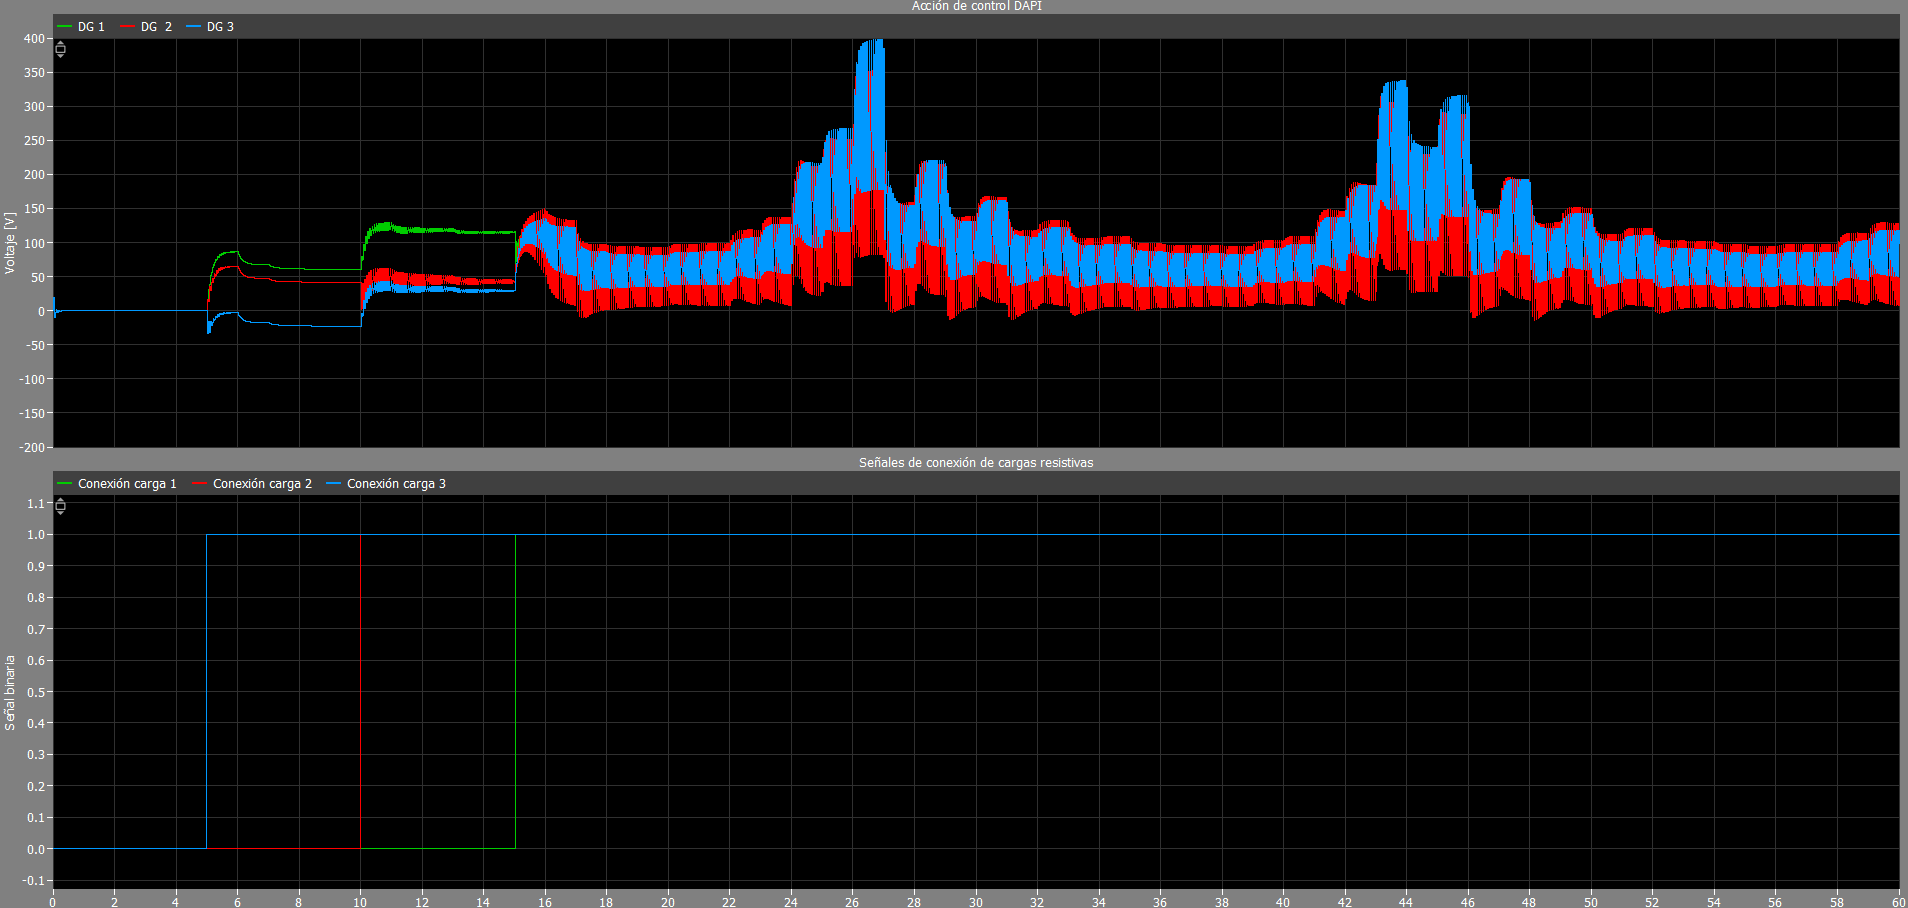
\includegraphics[width=1.0\linewidth]{Tarea 2/report/imagenes/p2a/accion_dapi_mal.png}
    \caption{Gráfico de voltajes de cada unidad de generación, junto a las señales de conexión/desconexión de cargas para una frecuencia de desacople de 2 Hz y una frecuencia del DAPI de 2 Hz.}
    \label{accion_dapi_mal}
\end{figure}

A partir de la simulación se puede observar un comportamiento inestable en los voltajes de las unidades generadoras, especialmente tras la conexión de las cargas resistivas. Aunque inicialmente los voltajes comienzan a estabilizarse, al conectarse más cargas, las unidades DG$_2$ y DG$_3$ muestran oscilaciones significativas, lo que sugiere que el controlador DAPI no está sintonizado correctamente para manejar las perturbaciones. Estas oscilaciones persistentes indican que el sistema está lejos de alcanzar el equilibrio, y el control DAPI no logra restaurar eficazmente los niveles de tensión, lo que podría llevar a problemas operativos si no se corrige.

\subsection{Parte b.-}

En esta sección se sintonizó el controlador DAPI utilizando la estrategia de \textit{trade-off}. Esta técnica de sintonización balancea los parámetros de la red, buscando un compromiso entre qué tan bien se comparten las potencias y los voltajes entres las unidades de generación. En la Figura \ref{potencia-compartida}, se observa, que teniendo un ponderador alto asociado a los errores de potencia en comparación al de voltaje, se tienen potencias muy similares independientemente de cuáles cargas están conectadas. Sin embargo, el voltaje tiene problemas para seguir el valor nominal de 400V, teniendo hasta 200V de diferencia de una unidad generadora a otra, como se puede observar en la Figura \ref{voltaje-malo}.

Por el otro lado, teniendo un ponderador alto para el error de voltaje versus uno bajo para los cuocientes de potencia, se tiene un seguimiento mejor de voltaje, como se puede observar en la Figura \ref{voltaje-compartido}, mientras que las potencias se comparten peor, como se puede observar en la Figura \ref{potencia-mala}, lo cual concuerda con el principio de \textit{trade-off} con el que se sintoniza el controlador. 
 
\begin{figure}
    \centering
    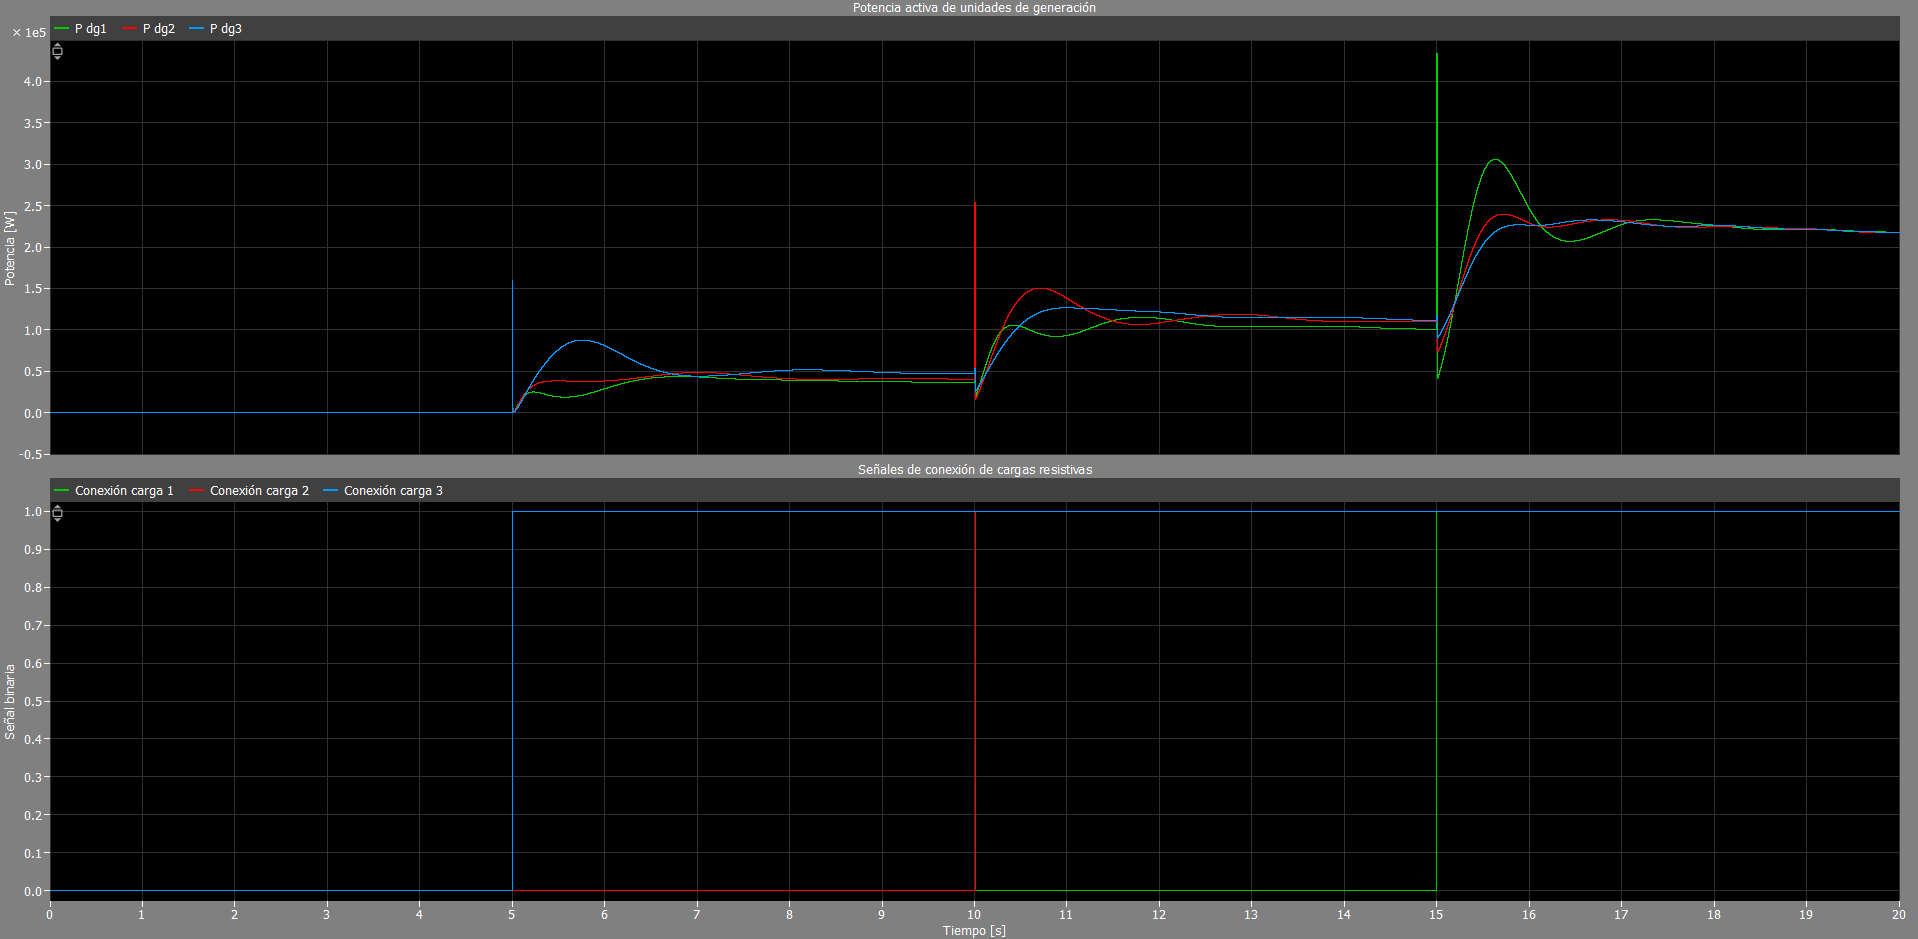
\includegraphics[width=0.5\linewidth]{Tarea 2/report/imagenes/p2b/potencia-compartida.png}
    \caption{Potencias de unidades generadoras con $\gamma = 0.5$ y matriz de adyacencia ponderada por $c = 10$.}
    \label{potencia-compartida}
\end{figure}

\begin{figure}
    \centering
    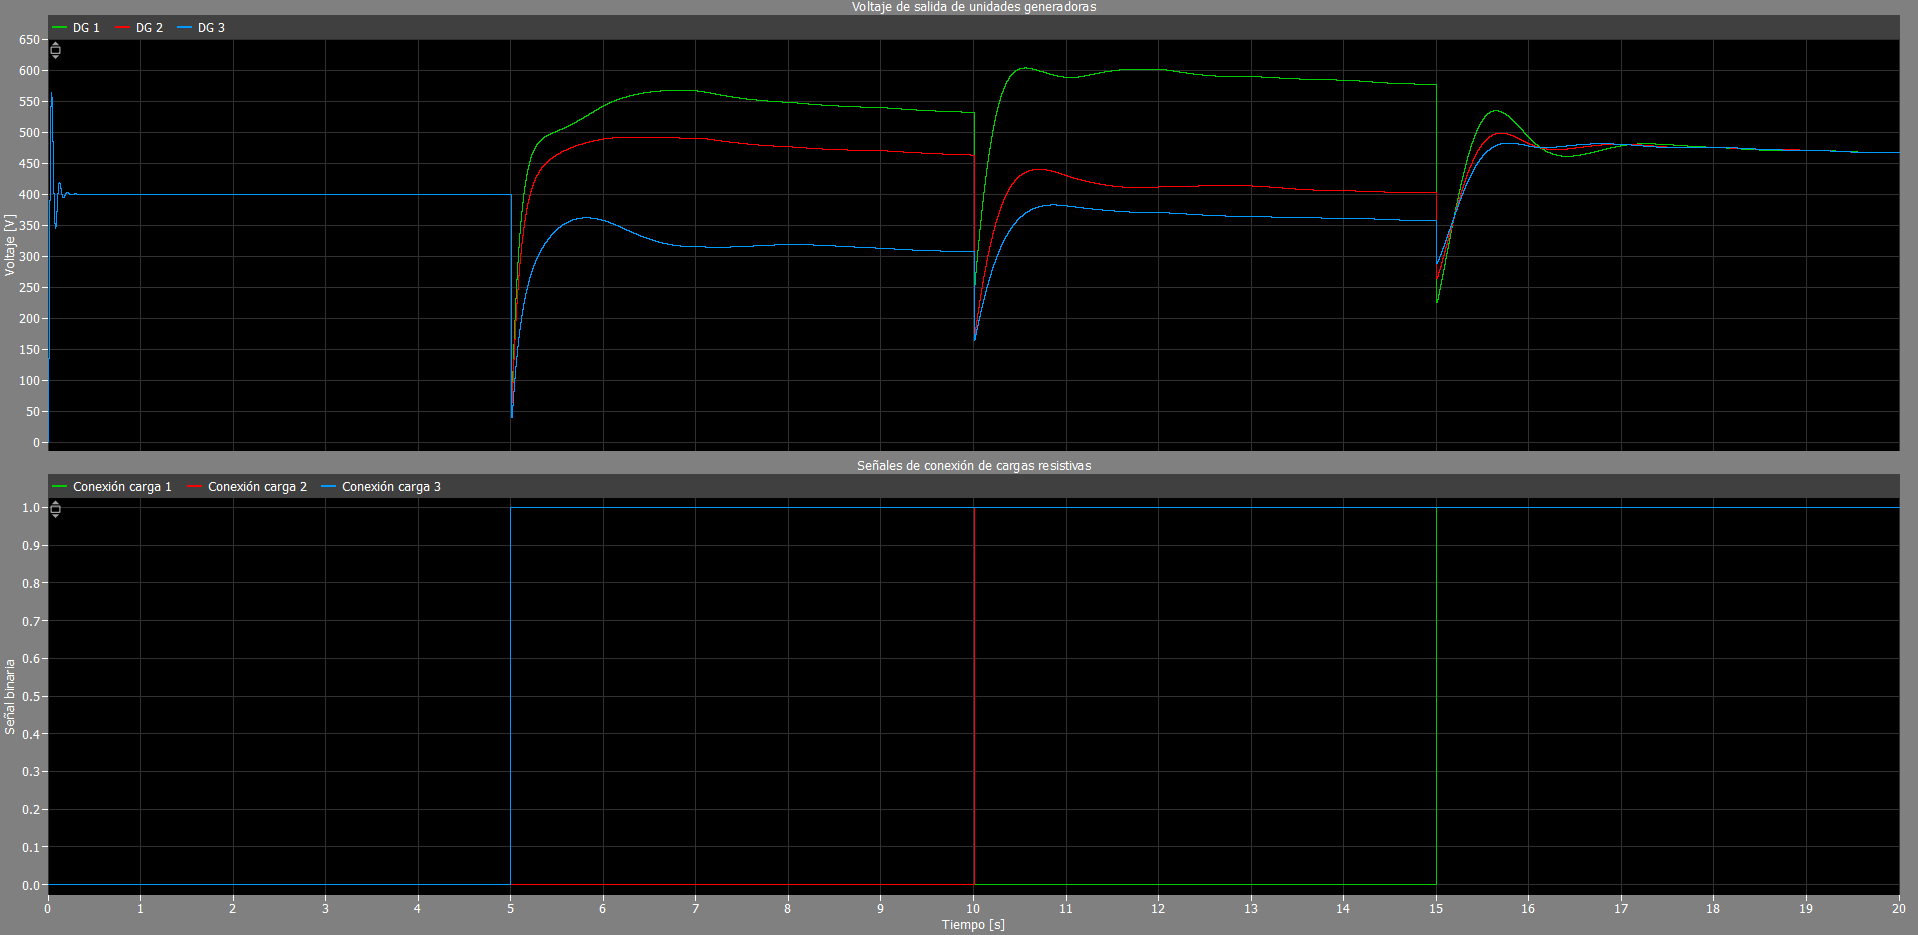
\includegraphics[width=0.5\linewidth]{Tarea 2/report/imagenes/p2b/voltaje-malo.png}
    \caption{Voltajes de unidades generadoras con $\gamma = 0.5$ y matriz de adyacencia ponderada por $c = 10$.}
    \label{voltaje-malo}
\end{figure}

\begin{figure}
    \centering
    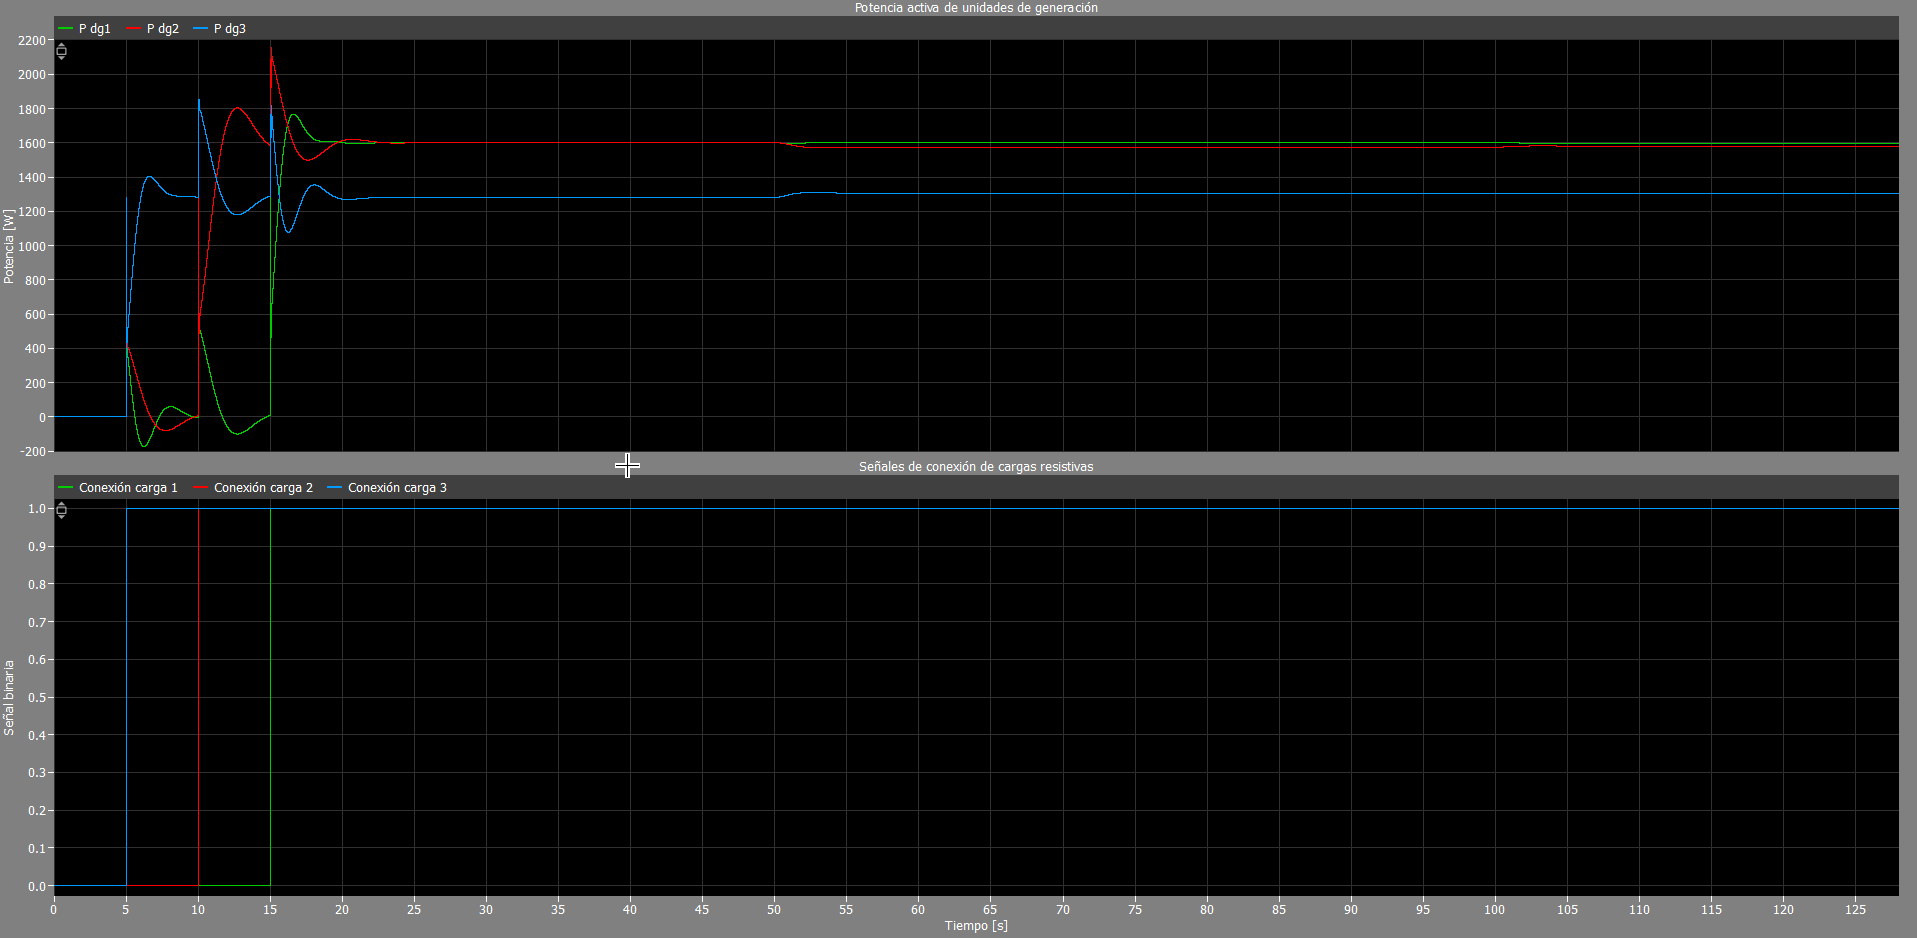
\includegraphics[width=0.5\linewidth]{Tarea 2/report/imagenes/p2b/potencia-mala.png}
    \caption{Potencias de unidades generadoras con $\gamma = 5$ y matriz de adyacencia ponderada por $c = 0.5$.}
    \label{potencia-mala}
\end{figure}

\begin{figure}
    \centering
    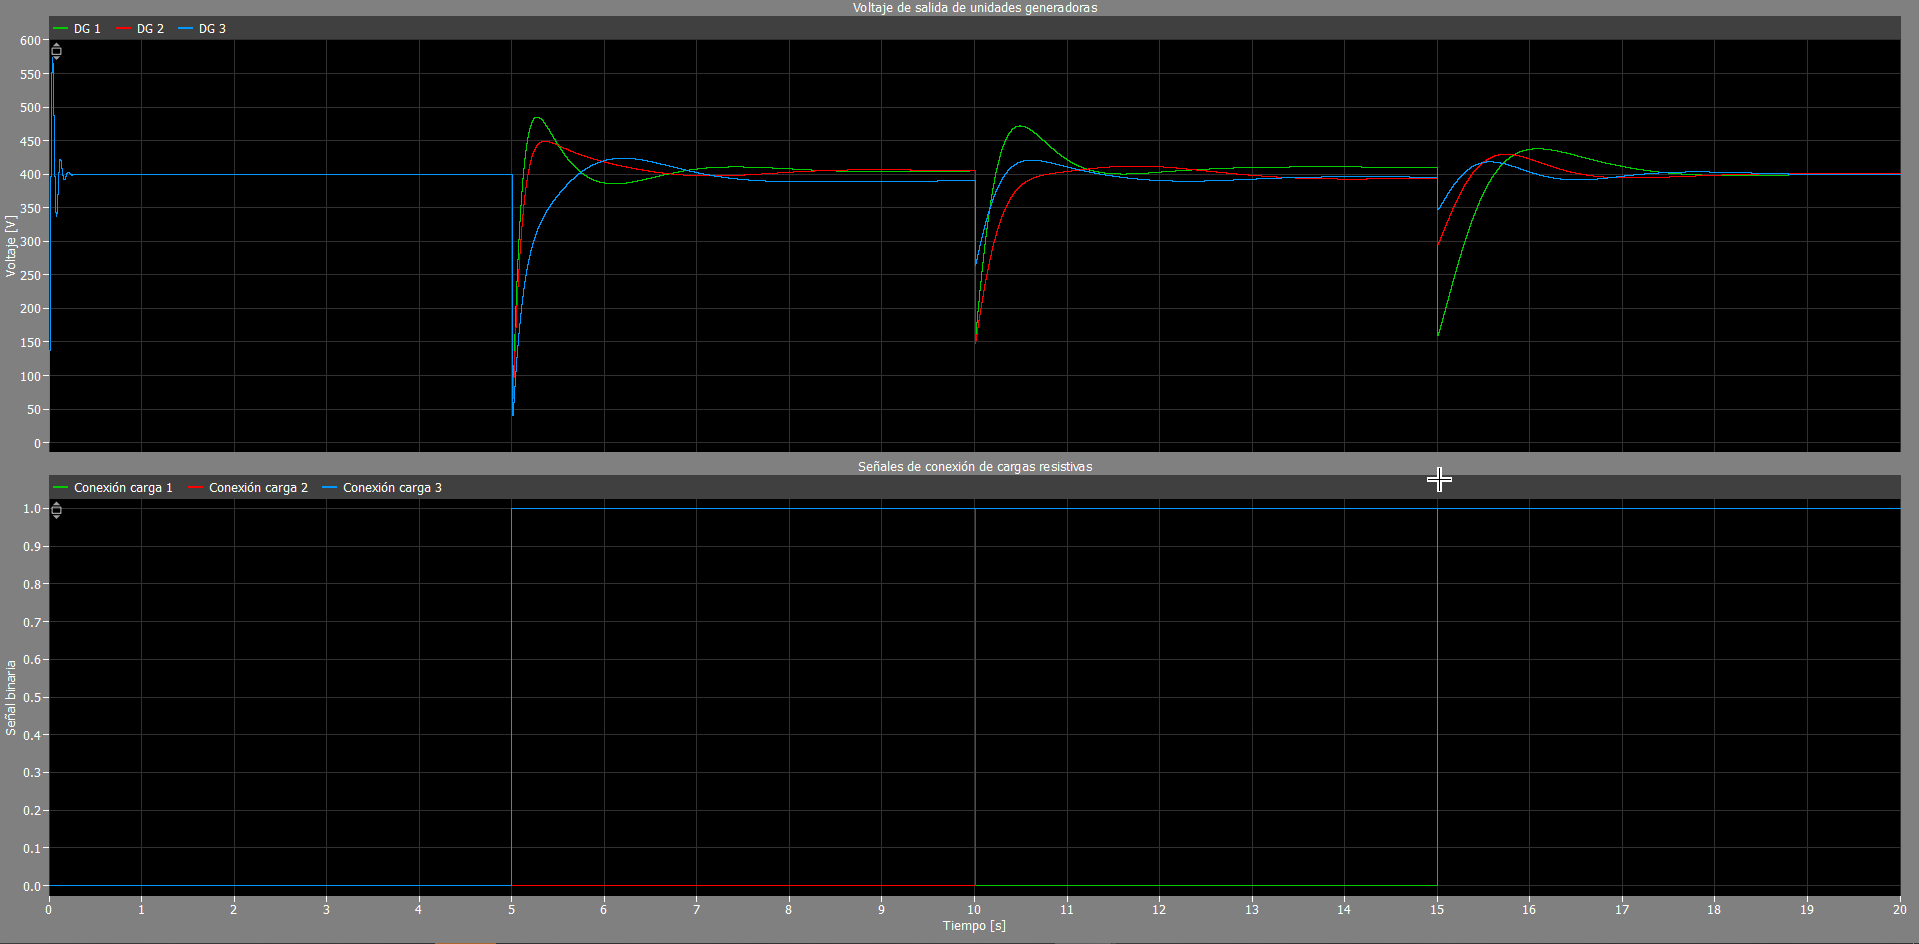
\includegraphics[width=0.5\linewidth]{Tarea 2/report/imagenes/p2b/voltaje-compartido.png}
    \caption{Potencias de unidades generadoras con $\gamma = 5$ y matriz de adyacencia ponderada por $c = 0.5$.}
    \label{voltaje-compartido}
\end{figure}


\begin{table}[h!]
\centering
\begin{tabular}{|c|c|c|c|}
\hline
 & DG 1 & DG 2 & DG 3 \\ 
\hline
$\gamma$ & 0.5 & 0.5 & 0.5 \\ 
\hline
$\zeta$  & 0.5 & 0.5 & 0.5 \\ 
\hline
\end{tabular}
\caption{Parámetros de sintonización de controlador DAPI.}
\label{parametros_dapi}
\end{table}

% Poner graficos que muestren los resultados de la sintonización

Al aplicar esta estrategia, se observó que la red logró un comportamiento más estable, con tiempos de respuesta más rápidos en comparación con la sintonización inicial. El ajuste de los parámetros del DAPI permitió que el sistema restaurara los niveles de tensión de manera más eficiente, sin generar sobreoscilaciones significativas ni picos de tensión indeseados. Aunque se sacrificó ligeramente la rapidez de la respuesta en algunos casos, el resultado fue un sistema más robusto frente a variaciones en la demanda de carga.\\

Los parámetros de interés, como el error en estado estacionario y la velocidad de convergencia de la tensión a su valor de referencia, mostraron mejoras considerables tras la sintonización mediante trade-off. En particular, el error en estado estacionario se redujo significativamente, lo que indica que el controlador fue capaz de corregir las desviaciones de tensión de manera precisa, incluso ante perturbaciones prolongadas en la red.

\subsection{Parte c.-}

%Para continuar, se utilizó la estrategia de \textit{Smart tuning} en la sintonización del controlador DAPI. Se seleccionó la unidad generadora 1 como unidad líder, y al resto como seguidoras. Los resultados obtenidos en esta sección se compararán con los de la estrategia de \textit{trade-off}, destacando los cambios en la respuesta del sistema y la mejora en la restauración de la tensión.

% Poner los resultados obtenidos por esta estrategia

%Tras la sintonización del controlador DAPI utilizando la estrategia de Smart tuning, se observó una mejora adicional en varios parámetros clave de la red en comparación con la estrategia de trade-off.\\

%Al aplicar Smart tuning, el sistema mostró una respuesta más rápida y precisa, reduciendo aún más el tiempo de recuperación de los niveles de tensión a sus valores de referencia. Además, se logró una disminución notable en el error en estado estacionario, lo que permitió que el sistema restaurara la tensión de manera más eficiente, con una mayor precisión en comparación con la estrategia de trade-off. Las oscilaciones presentes en la tensión también se redujeron, mejorando la estabilidad general de la red.\\

%En cuanto a las diferencias observadas entre ambas estrategias, Smart tuning permitió una respuesta más agresiva sin comprometer la estabilidad del sistema. Mientras que la estrategia de trade-off ofrecía un balance entre velocidad y estabilidad, Smart tuning maximizó ambos factores, consiguiendo una restauración de tensión más rápida y con menos oscilaciones. Sin embargo, esto implicó un proceso de ajuste más automatizado y refinado, que podría no ser tan sencillo de aplicar manualmente en todos los sistemas como lo es trade-off.

\subsection{Parte d.-}

Finalmente, se analizó el impacto de modificar el tiempo de muestreo del control secundario sobre el desempeño del sistema. Esta variación en el tiempo de muestreo puede afectar la estabilidad y la velocidad de respuesta del controlador DAPI.\\

Como se observa en la Figura \ref{sampling_bajo} el tiempo de muestreo se redujo, el controlador pudo reaccionar más rápidamente ante las perturbaciones en la red, mejorando el tiempo de respuesta del sistema y minimizando los errores transitorios. Sin embargo, si el tiempo de muestreo se reduce excesivamente, puede haber un incremento en el consumo de recursos computacionales, lo que podría no ser viable en aplicaciones prácticas donde la capacidad de procesamiento es limitada, especialmente considerando las alternativas actuales de comunicación entre unidades de generación. Además, tiempos de muestreo muy pequeños pueden introducir ruido en las mediciones y generar oscilaciones indeseadas en la respuesta del sistema, comprometiendo la estabilidad.\\

Por otro lado, como se observa en la Figura \ref{sampling_alto}, cuando se incrementó el tiempo de muestreo el sistema mostró una respuesta más lenta a las perturbaciones, lo que incrementó el tiempo necesario para alcanzar el estado estacionario. Aunque esto puede aliviar la carga computacional del sistema, el principal efecto negativo fue la disminución de la capacidad del controlador para responder rápidamente.

\begin{figure}
    \centering
    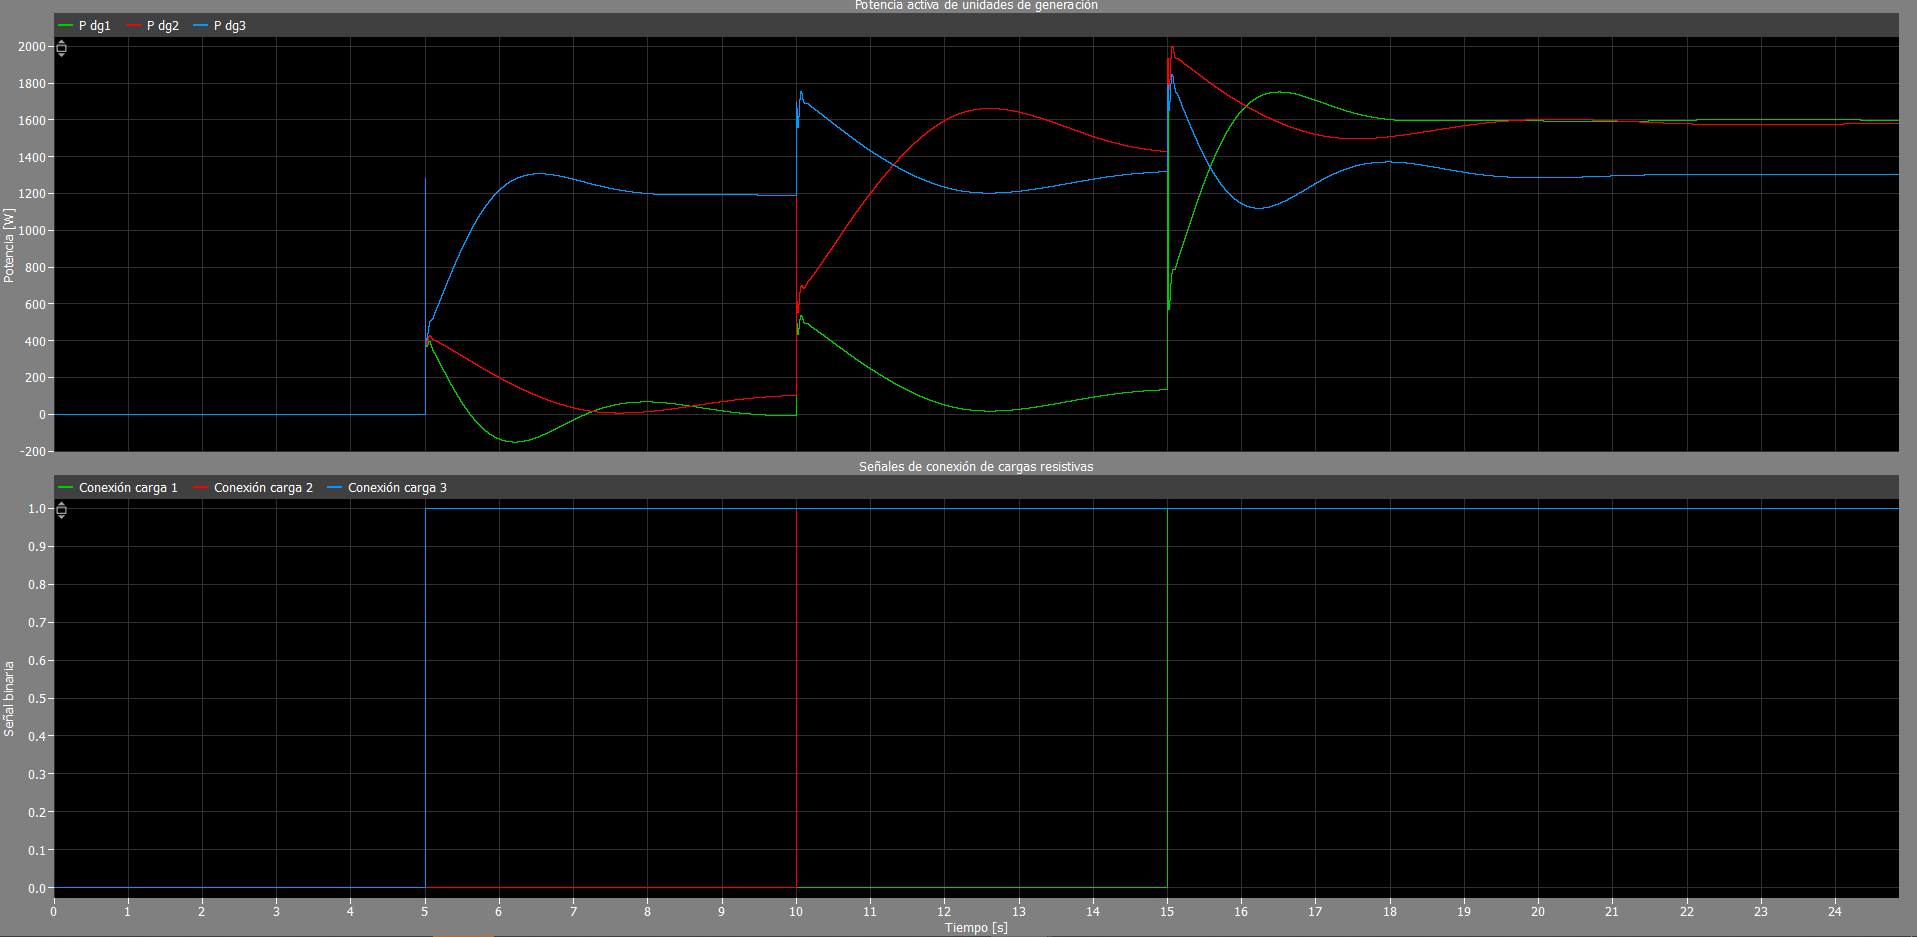
\includegraphics[width=0.5\linewidth]{Tarea 2/report/imagenes/p2b/sampling_bajo.png}
    \caption{Potencias de unidades generadoras con tiempo de muestreo de 1 segundo.}
    \label{sampling_bajo}
\end{figure}

\begin{figure}
    \centering
    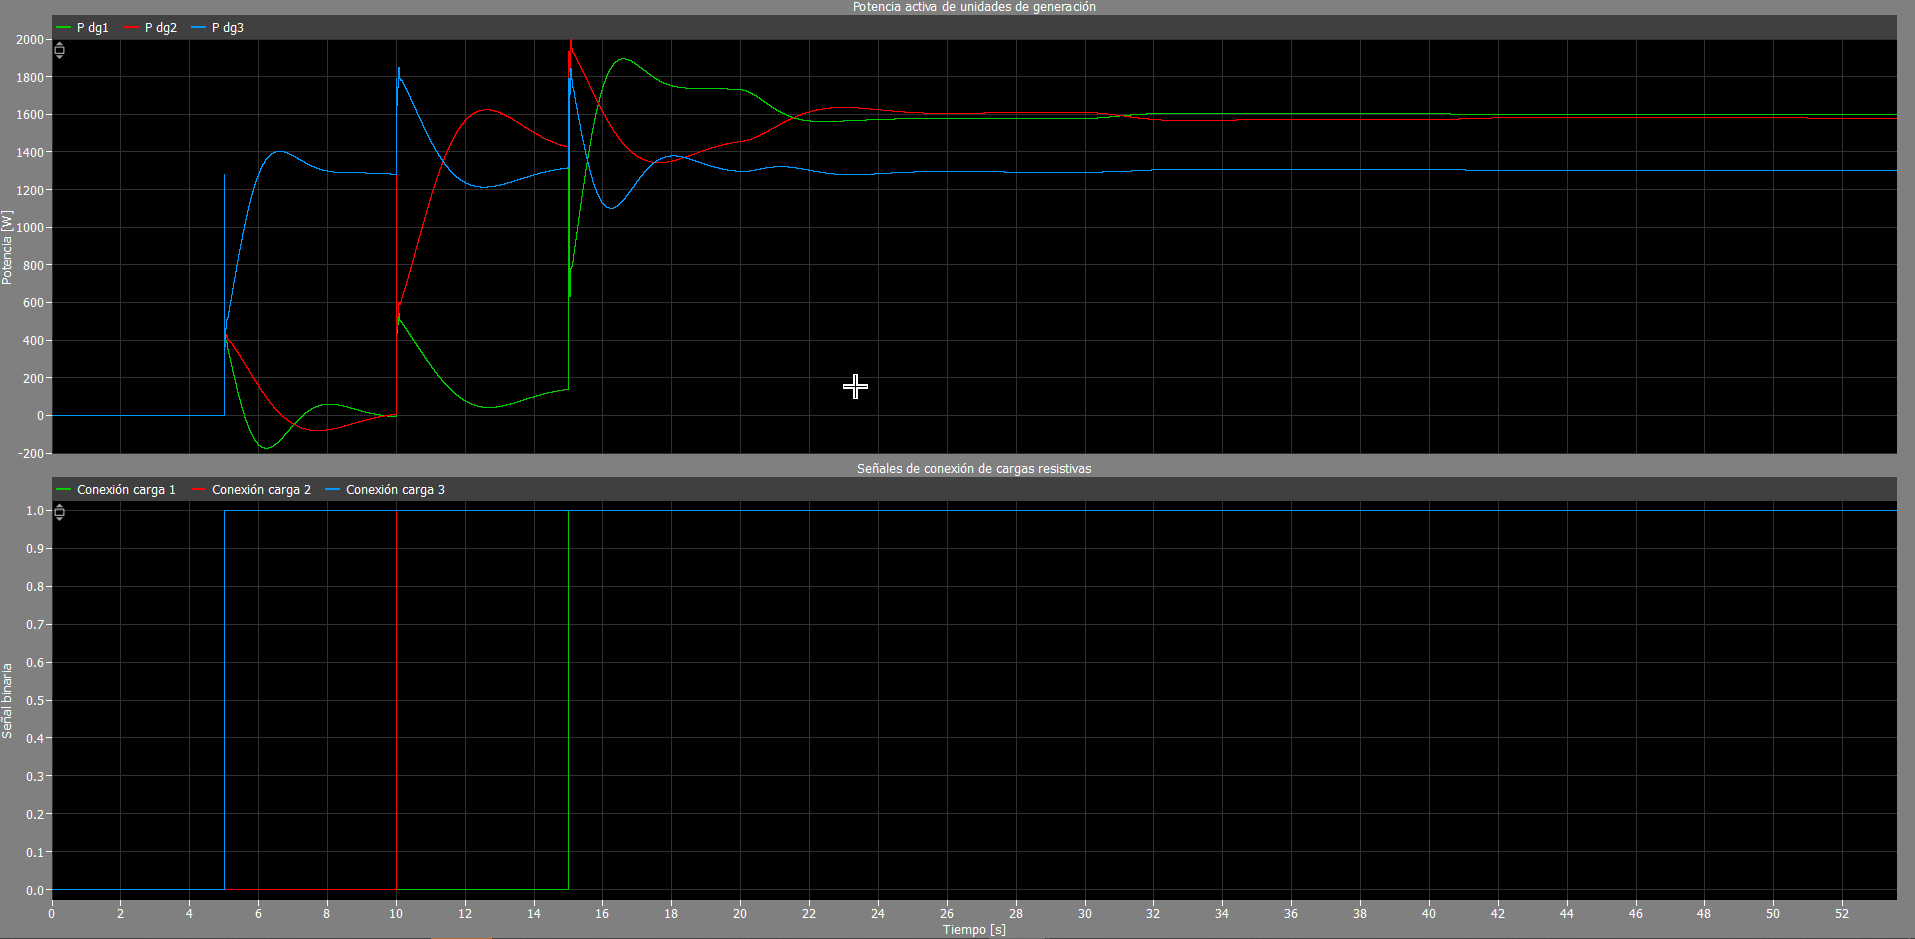
\includegraphics[width=0.5\linewidth]{Tarea 2/report/imagenes/p2b/sampling_alto.png}
    \caption{Potencias de unidades generadoras con tiempo de muestreo de 1 segundo.}
    \label{sampling_alto}
\end{figure}

\section{Pregunta 3}

\subsection{Parte a.-}

El primer escenario de prueba consistió en observar el impacto de la carga sobre el controlador al conectar y desconectar cargas en la micro-red. Este escenario es crucial para evaluar la robustez del sistema y la capacidad del controlador para mantener los niveles de tensión dentro de los rangos establecidos.\\

La simulación se inició con todas las unidades de generación DC encendidas y completamente comunicadas, garantizando que el sistema estuviera en equilibrio antes de aplicar las perturbaciones. Posteriormente, se conectaron una a una las cargas del sistema, y una vez alcanzada la máxima demanda, se procedió a desconectar las cargas de manera inversa, es decir, desconectándolas gradualmente hasta eliminar por completo la demanda. De aquí se obtienen las Figuras \ref{potencia_desconexion} y \ref{voltaje_desconexion}.

% Poner resultados para cada escenario

Los resultados de la simulación muestran que, al agregar cargas, el controlador DAPI respondió de manera eficiente, ajustando la potencia entregada por las unidades de generación para mantener la tensión dentro de los niveles de referencia. A medida que se incrementaba la demanda, las unidades de generación adaptaban su potencia de manera proporcional, y el controlador mantuvo la estabilidad de la red sin generar fluctuaciones significativas en la tensión. En particular, se observa que la potencia se compartió mejor entre las unidades con cargas conectadas directamente a ellas. \\


\begin{figure}
    \centering
    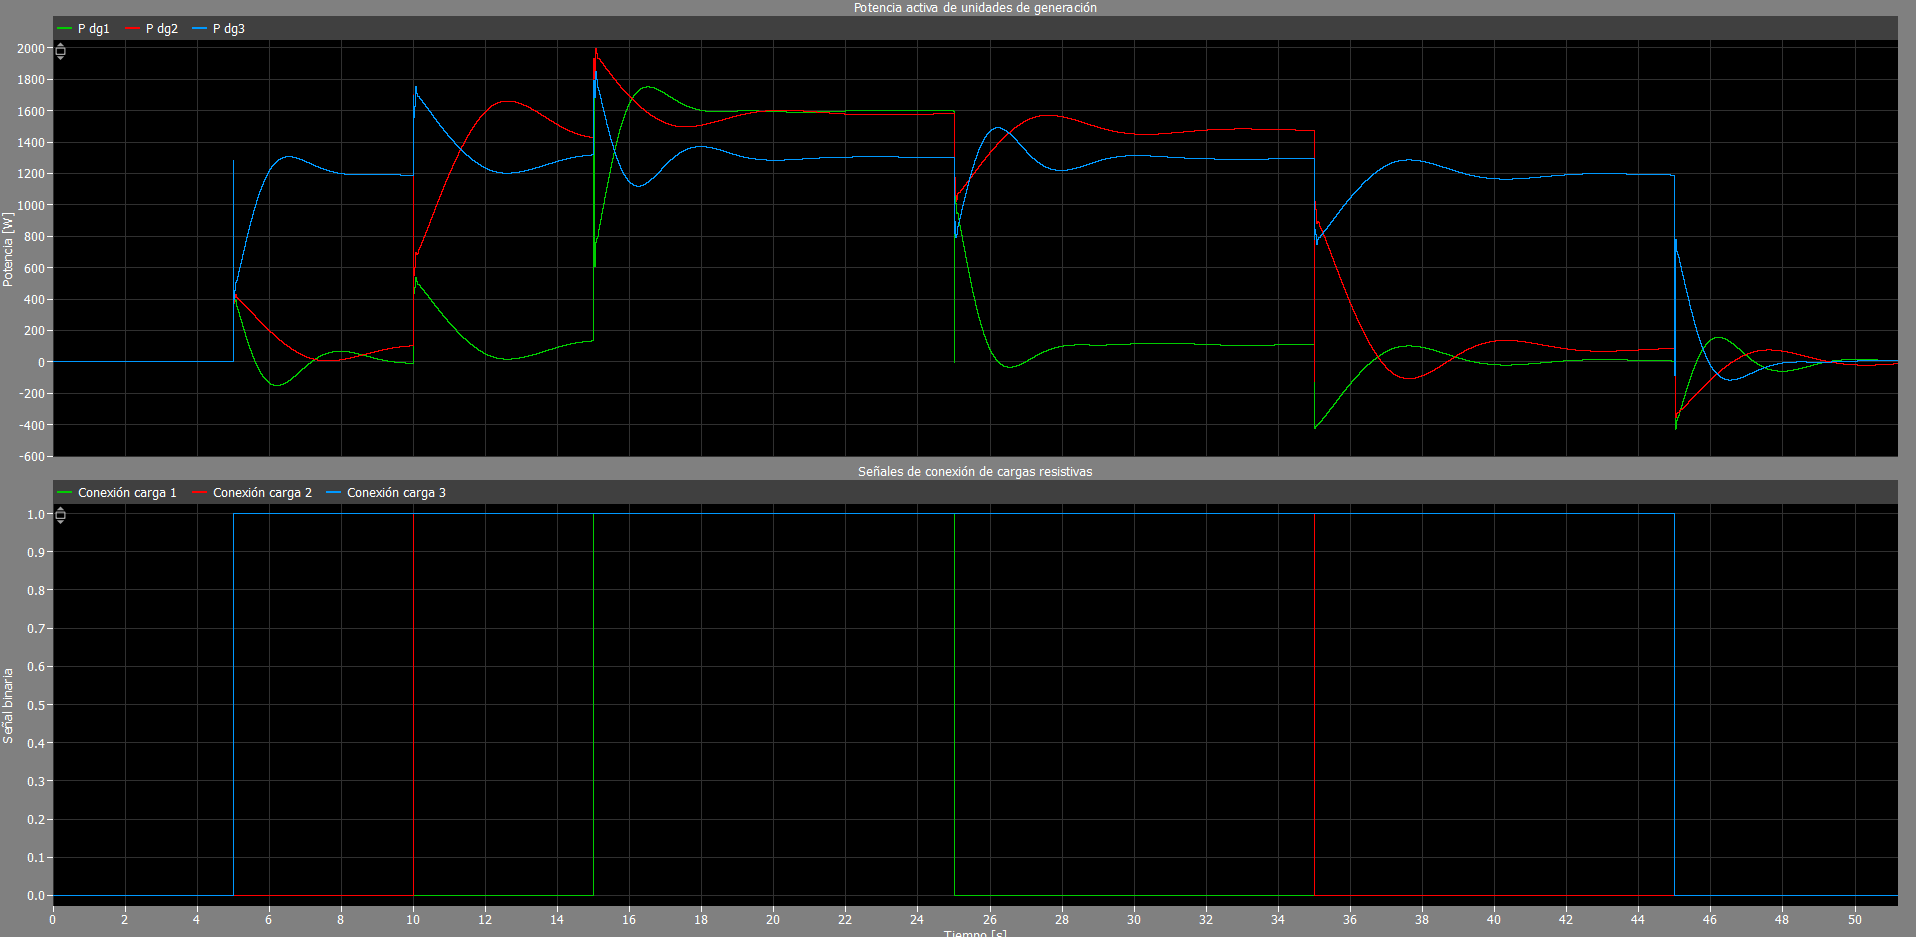
\includegraphics[width=0.5\linewidth]{Tarea 2/report/imagenes/p3a/potencia.png}
    \caption{Potencias de unidades generadoras frente a conexión y desconexión de cargas.}
    \label{potencia_desconexion}
\end{figure}

\begin{figure}
    \centering
    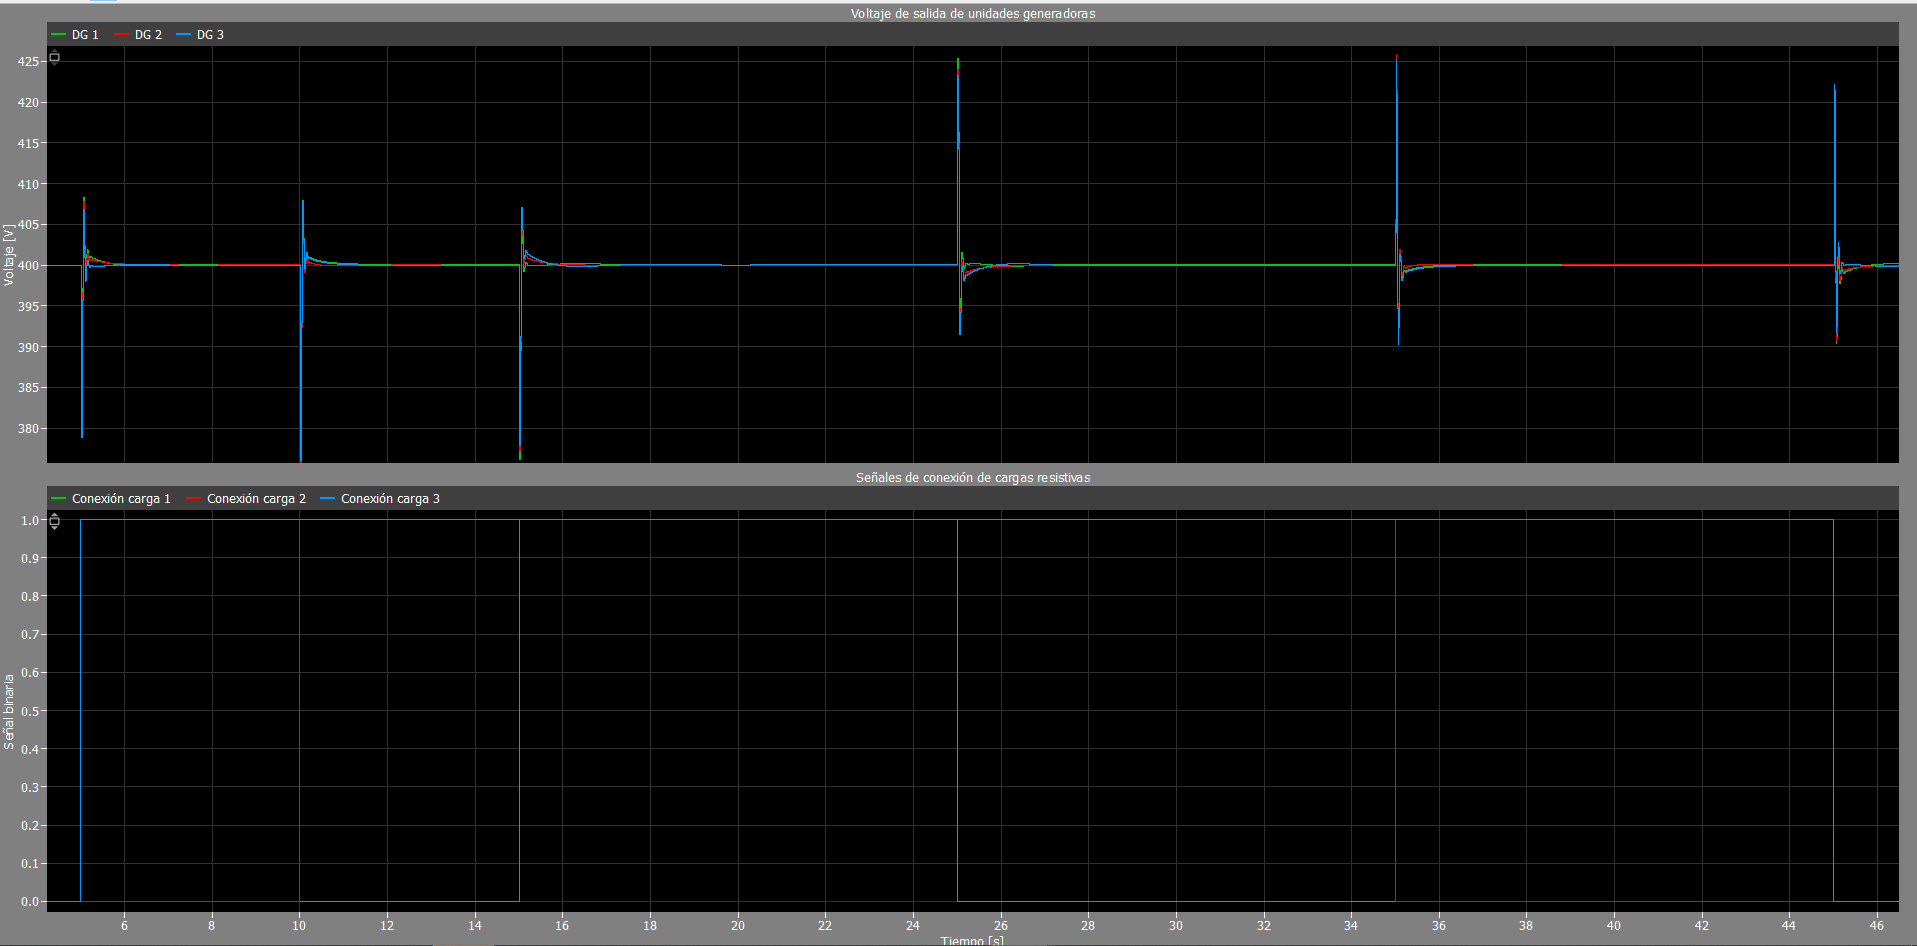
\includegraphics[width=0.5\linewidth]{Tarea 2/report/imagenes/p3a/voltajes.png}
    \caption{Voltajes de unidades generadoras frente a conexión y desconexión de cargas.}
    \label{voltaje_desconexion}
\end{figure}


Cuando se comenzó a desconectar las cargas, el sistema reaccionó de manera inversa, reduciendo la potencia entregada por las unidades de generación. El controlador fue capaz de ajustar la salida de potencia de manera proporcional a la reducción de demanda, logrando restaurar los niveles de tensión a sus valores de referencia sin sobreoscilaciones. Durante este proceso, el sistema mostró una estabilidad robusta, sin pérdidas notables en el control de la tensión.

\subsection{Parte b.-}

Se simuló el efecto de un retardo comunicacional entre los nodos de control de las unidades generadoras. Este retardo, que varía de 1 a 20 veces el tiempo de muestreo del control secundario, permite evaluar el impacto de las demoras en la comunicación sobre la estabilidad y eficiencia del sistema. Los resultados de la simulación mostrarán cómo los distintos niveles de retardo afectan el control de la micro-red.

\subsubsection{Retardo de 1 vez el tiempo de muestreo del control secundario - X segundos}

% Poner resultados de esta sección

Los resultados mostraron que con un retardo de 1 vez el tiempo de muestreo, el sistema continuó operando de manera estable, con una mínima afectación en el tiempo de respuesta del controlador. Aunque hubo una leve demora en la corrección de los niveles de tensión tras las variaciones de carga, el sistema logró restaurar la tensión a los valores de referencia sin mayores complicaciones. Los resultados de esta parte corresponden a aquellos de las Figuras \ref{potencia_desconexion} y \ref{voltaje_desconexion}.

\subsubsection{Retardo de 20 veces el tiempo de muestreo del control secundario - W segundos}

% Poner resultados de esta sección

Finalmente, con un retardo de 20 veces el tiempo de muestreo, el sistema presentó una inestabilidad considerable. Los nodos de control tardaban demasiado en recibir la información necesaria para ajustar la potencia de las unidades generadoras, lo que provocó fluctuaciones severas en los niveles de tensión. En algunos casos, el sistema fue incapaz de restaurar los niveles de tensión de manera efectiva, evidenciando la crítica influencia de grandes retardos en la comunicación sobre la estabilidad del sistema.\\

De manera general, se puede notar que si bien retardos pequeños pueden ser manejados de manera efectiva, aumentos sustanciales en el retardo comunicacional resultan en una degradación notable del desempeño del sistema, lo que puede comprometer la estabilidad y la respuesta del controlador ante variaciones de carga.

\subsection{Parte c.-}

En este escenario, se emularon fallas de comunicación entre las unidades de generación DC, cortando de uno en uno los canales de comunicación. El objetivo es observar cómo el sistema responde ante la pérdida de comunicación y qué efecto tiene esto sobre la estabilidad del control de la micro-red. Los resultados permitirán identificar las vulnerabilidades del sistema ante fallos comunicacionales.

% Poner resultados de esta sección

Los resultados mostraron que al cortar un solo canal de comunicación, el sistema fue capaz de mantener un control relativamente estable de la micro-red, aunque la coordinación entre las unidades generadoras se vio afectada. El controlador DAPI, utilizando los canales restantes, logró compensar la pérdida, y aunque hubo un pequeño aumento en el tiempo de respuesta para restaurar los niveles de tensión, el sistema no mostró signos significativos de inestabilidad.\\

A medida que se cortaron más canales de comunicación, la capacidad del sistema para distribuir de manera eficiente la potencia entre las unidades generadoras disminuyó. Con dos canales fuera de operación, se observó un aumento en las oscilaciones de tensión y una reducción en la precisión con la que las unidades generadoras ajustaban su potencia. Aunque el sistema seguía siendo capaz de restaurar la tensión de manera eventual, la respuesta se hizo más lenta y menos eficiente.\\

Cuando se cortaron tres o más canales, el sistema comenzó a mostrar signos claros de inestabilidad. La pérdida de comunicación entre las unidades de generación dificultó la capacidad del controlador DAPI para coordinar la distribución de la potencia, lo que resultó en fluctuaciones más severas de la tensión y en algunos casos, picos de tensión no deseados. En estos escenarios, el sistema tardó considerablemente más en restaurar los niveles de tensión, y las oscilaciones en la red se volvieron más pronunciadas.\\

Finalmente, cuando se cortaron todos los canales de comunicación, el sistema fue incapaz de restaurar la tensión de manera efectiva. La falta de coordinación entre las unidades generadoras provocó un desbalance significativo en la distribución de la potencia, lo que llevó a fluctuaciones extremas en los niveles de tensión y, en algunos casos, fallas en la operación de la micro-red.

\subsection{Parte d.-}

Finalmente, se simuló la desconexión de una unidad de generación de la red, emulando una falla o desconexión programada. Posteriormente, se reconectó la unidad al sistema para analizar el impacto que esto tiene sobre el control de la micro-red. Los resultados obtenidos en esta simulación proporcionarán información sobre la capacidad de recuperación del sistema ante fallas de unidades generadoras.

\subsubsection{Desconexión de una unidad de generación}

% Poner resultados de esta sección

Al desconectar una de las unidades generadoras, el sistema reaccionó ajustando la potencia entregada por las unidades restantes. Los resultados mostraron que, aunque la micro-red fue capaz de continuar operando sin interrupciones mayores, la tensión experimentó una ligera caída inicial debido a la pérdida de capacidad de generación. Las dos unidades restantes debieron compensar el déficit de potencia, lo que generó un incremento en su carga de trabajo. Este fenómeno se reflejó en un aumento en la potencia generada por cada unidad restante, lo que permitió mantener el suministro de energía a las cargas conectadas.\\

Sin embargo, la reducción en el número de unidades generadoras activas también disminuyó la redundancia en el sistema, lo que podría hacer que la red sea más vulnerable a perturbaciones adicionales. A pesar de esto, el controlador DAPI fue capaz de ajustar la salida de potencia de manera eficiente, restaurando la tensión a niveles cercanos a los de referencia tras la desconexión de la unidad, aunque con una respuesta más lenta y un pequeño margen de error en comparación con el escenario donde todas las unidades estaban conectadas.

\subsubsection{Reconexión de la unidad de generación}

% Poner resultados de esta sección

Una vez reconectada la unidad de generación al sistema, el controlador DAPI restableció rápidamente el equilibrio de potencia, redistribuyendo la carga entre las tres unidades generadoras. Los resultados mostraron que, tras la reconexión, la tensión volvió rápidamente a sus niveles de referencia y el sistema recuperó su estado normal de operación, con una distribución más uniforme de la potencia entre las tres unidades generadoras.\\

El proceso de reconexión no generó oscilaciones importantes en la tensión, lo que indica que el controlador DAPI fue capaz de manejar de manera eficiente tanto la desconexión como la reconexión de las unidades de generación. Este resultado valida la capacidad del controlador para adaptarse a eventos como fallas temporales o desconexiones programadas de generadores, garantizando la continuidad operativa de la micro-red sin comprometer la estabilidad.

---------------------------------------------------


De acuerdo a lo visto en clases, para calcular la pendiente droop para cada potencia se debe seguir las siguientes fórmulas:

\begin{equation}
    M_p = \frac{\Delta w}{P_{máx}}
\end{equation}

\begin{equation}
    M_q = \frac{\Delta w}{Q_{máx}}
\end{equation}

En nuestra implementación se optó por crear un subsistema con parámetros regulables a través del diálogo de la figura \ref{dialogo_dg}, por lo que se usa internamente las siguientes fórmulas:

\begin{equation*}    
M_p = -\omega_0\frac{(\Delta_\omega)}{100\cdot P_{max}};
\end{equation*}

\begin{equation*}
M_q = -V_0\frac{(\Delta_V)}{100\cdot Q_{max}};
\end{equation*}

donde $\Delta_V$ y $\Delta_\omega$ son valores dentro de los rangos estipulados en el enunciado de la tarea: $[0.1 - 30]$ para la frecuencia; $[0.1 - 10]$ para la tensión. Se consideró inicialmente una variación de frecuencia de 5\% y de voltaje de 2\%, obteniéndose las pendientes droop $M_p = -1.6\cdot 10^{-4}$ y $ Mq = -7.33 \cdot 10^{-4}$.\\

\begin{figure}
   \centering
   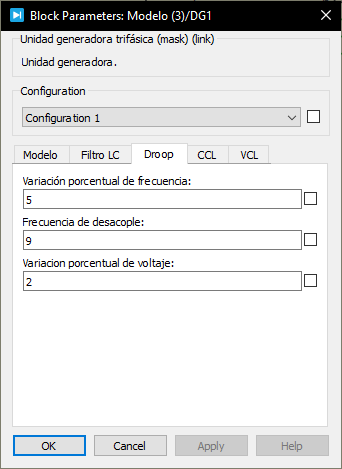
\includegraphics[width=0.5\linewidth]{Tarea 1/report/imagenes/p2a/dialogo_dg.png}
   \caption{Diálogo de parametrización de variables \textit{droop}.}
   \label{dialogo_dg}
\end{figure}

Al realizar una simulación teniendo las 3 máquinas generadoras con la misma pendiente droop de potencia activa y reactiva, se obtuvieron los siguientes resultados:

\begin{figure}
   \centering
   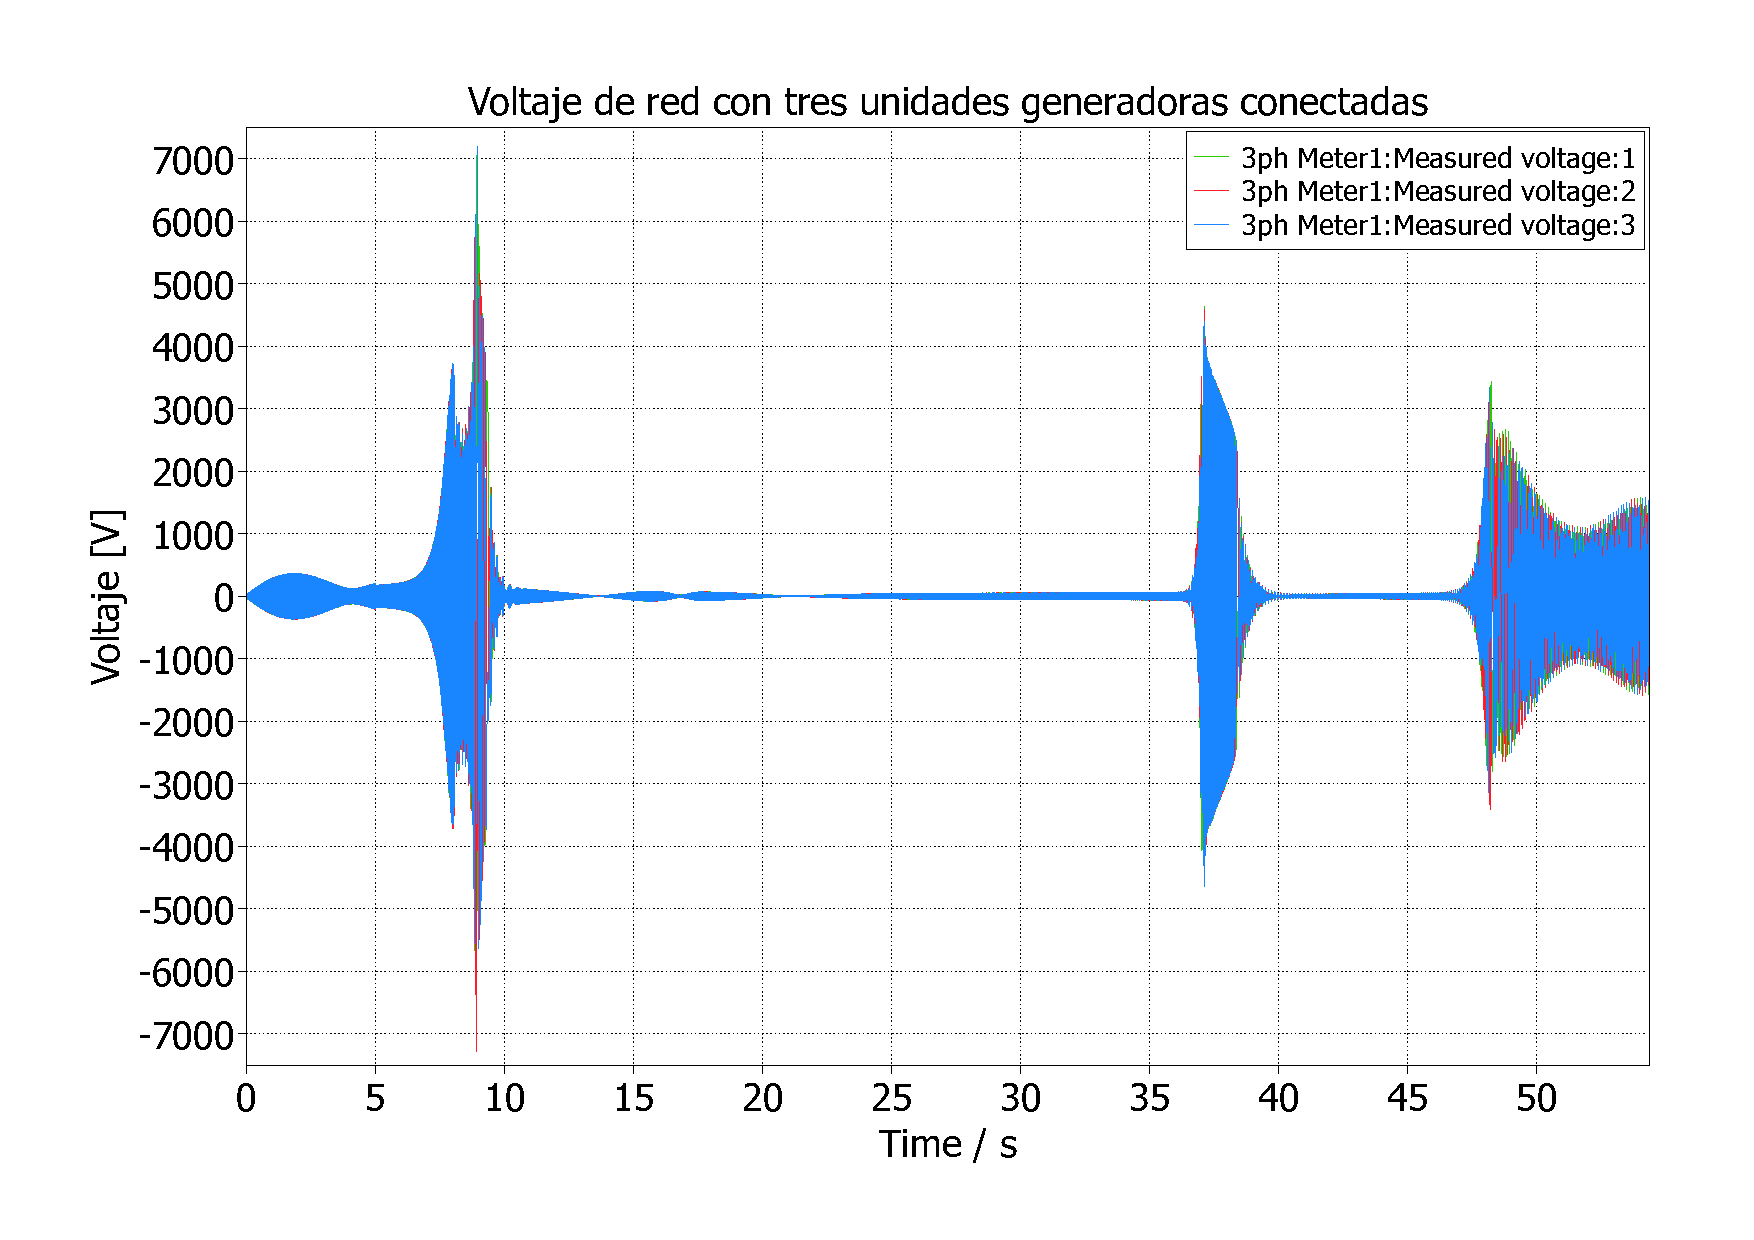
\includegraphics[width=0.5\linewidth]{Tarea 1/report/imagenes/p3a/resonancia_generadores.pdf}
   \caption{Diálogo de parametrización de variables \textit{droop}.}
   \label{resonancia_generadores}
\end{figure}

Se observa en la figura \ref{resonancia_generadores} que los generadores no logran mantener el voltaje dentro de un rango razonable en torno al voltaje nominal, que es lo que se hubiera esperado. Debido a esto, resulta imposible estudiar el efecto de la conexión y desconexión de cargas. Sin embargo, se puede estudiar el efecto del cambio de las pendientes \textit{droop} de una sola unidad generadora. A partir de esto se obtienen las figuras \ref{droop_1}, \ref{droop_2} y \ref{droop_3}, de las cuales no se puede apreciar cambios significativos.


\begin{figure}
   \centering
   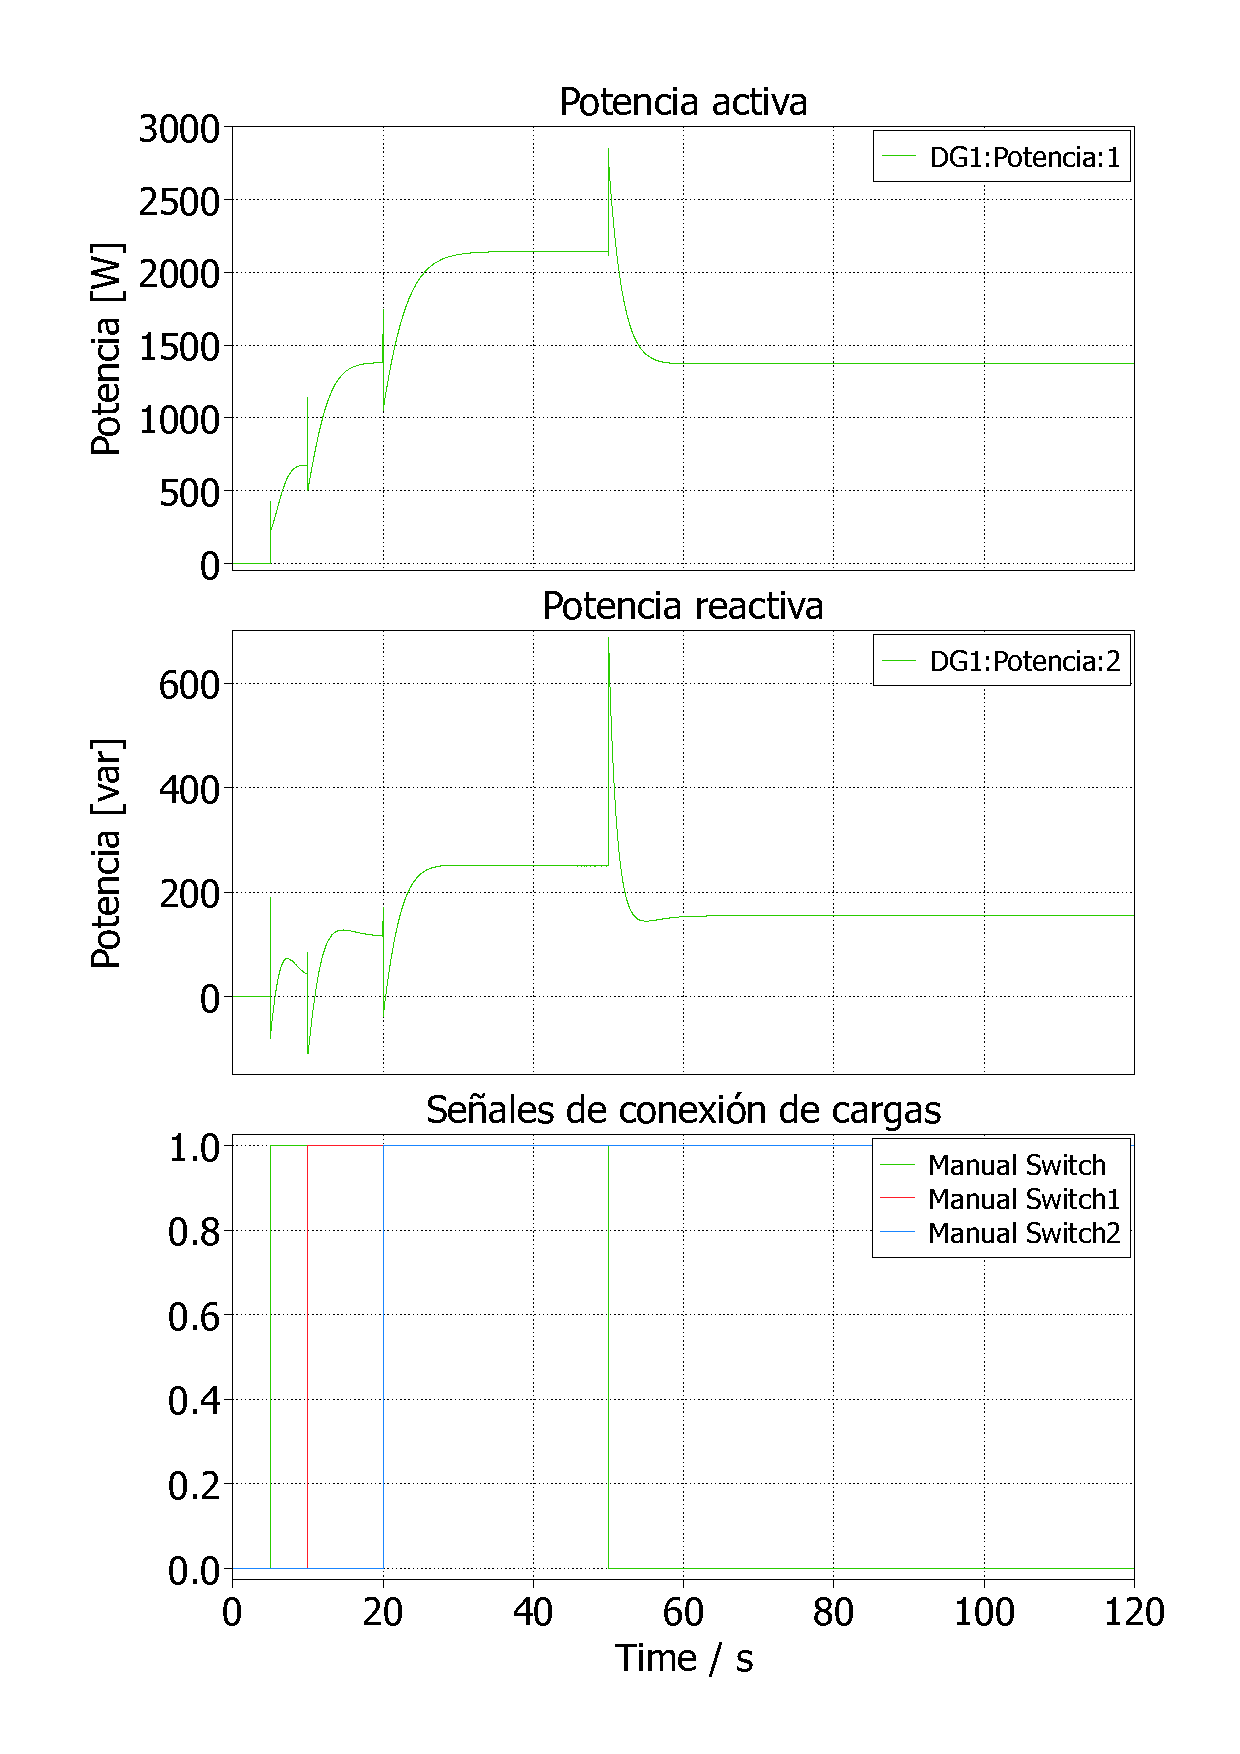
\includegraphics[width=0.5\linewidth]{Tarea 1/report/imagenes/p3a/droop_1.pdf}
   \caption{Potencia calculada con $Mp = -0.0005$ y $Mq_-0.0018$.}
   \label{droop_1}
\end{figure}

\begin{figure}
   \centering
   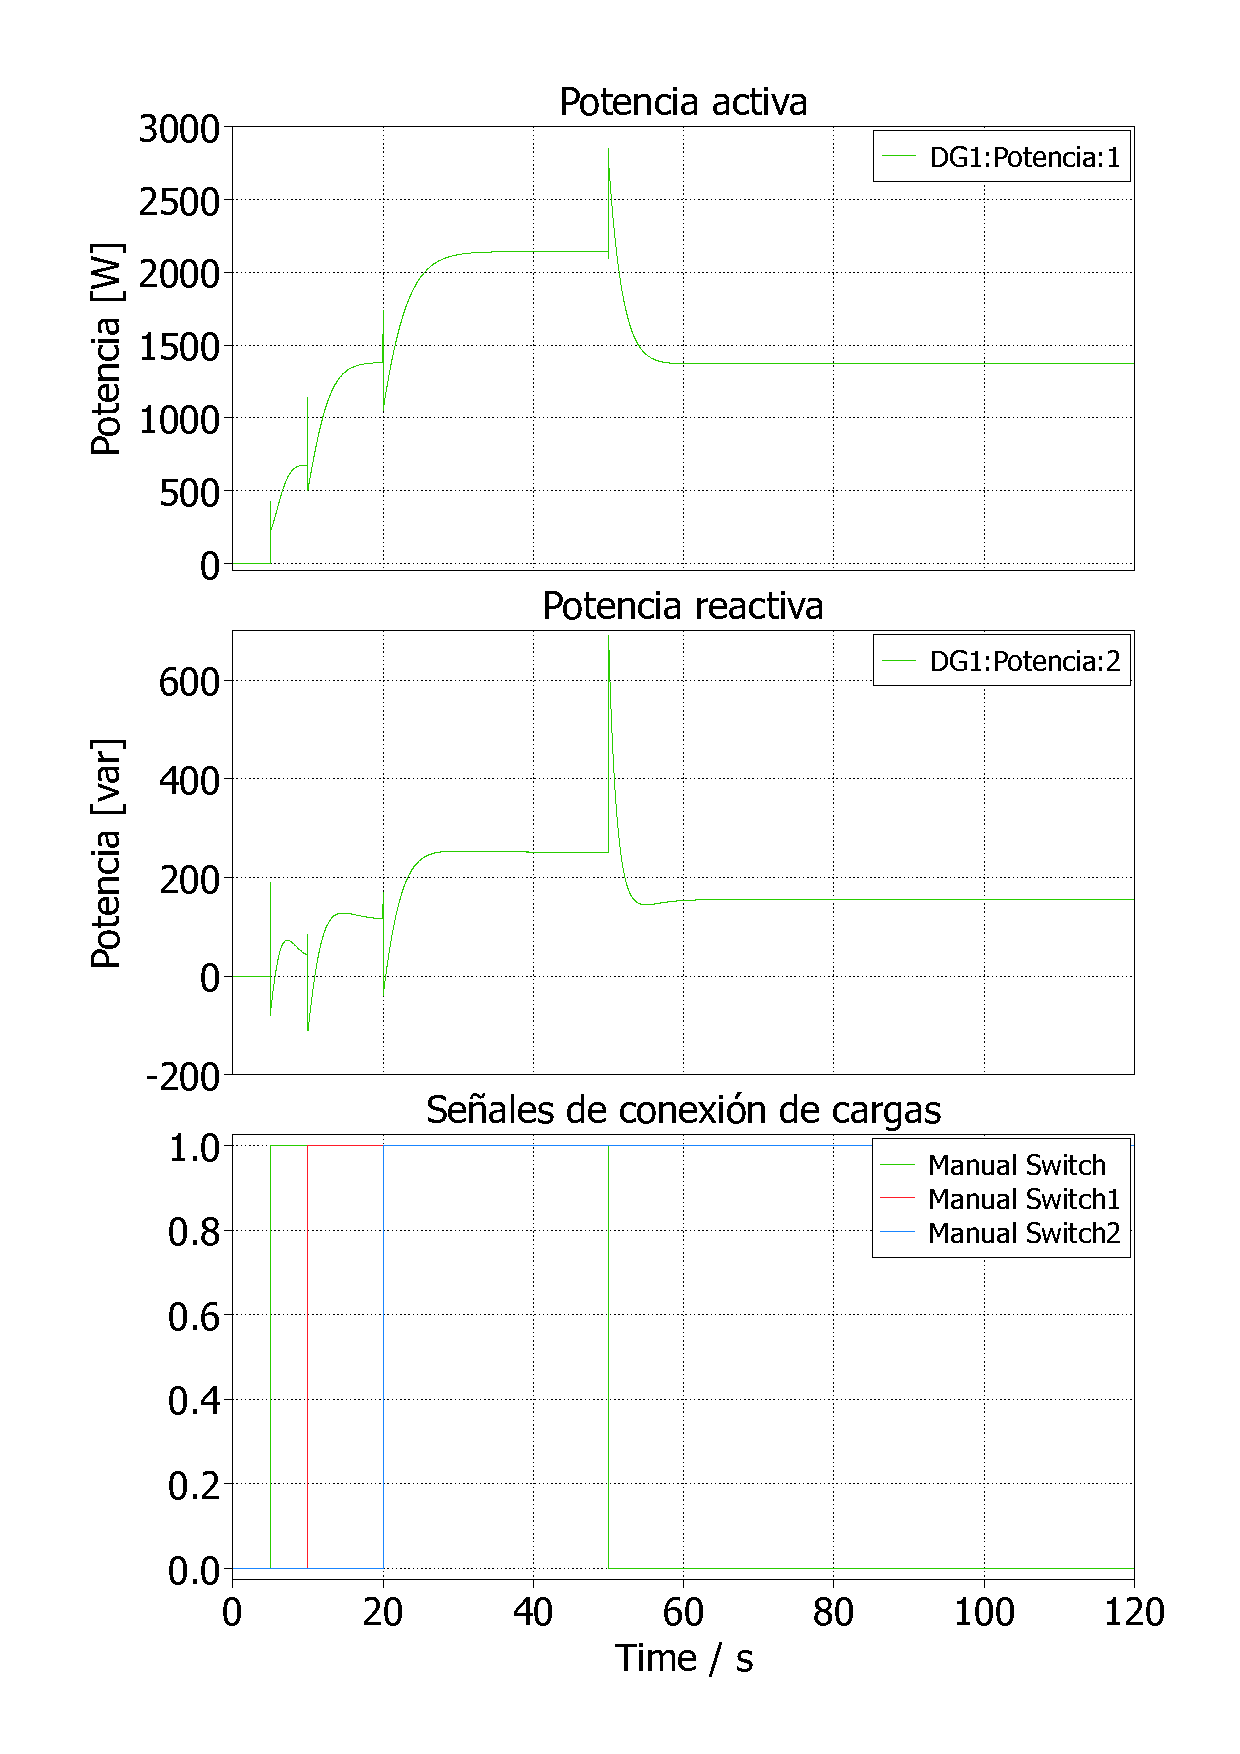
\includegraphics[width=0.5\linewidth]{Tarea 1/report/imagenes/p3a/droop_2.pdf}
   \caption{Potencia calculada con $Mp = -0.0003$ y $Mq_-0.0018$.}
   \label{droop_2}
\end{figure}

\begin{figure}
   \centering
   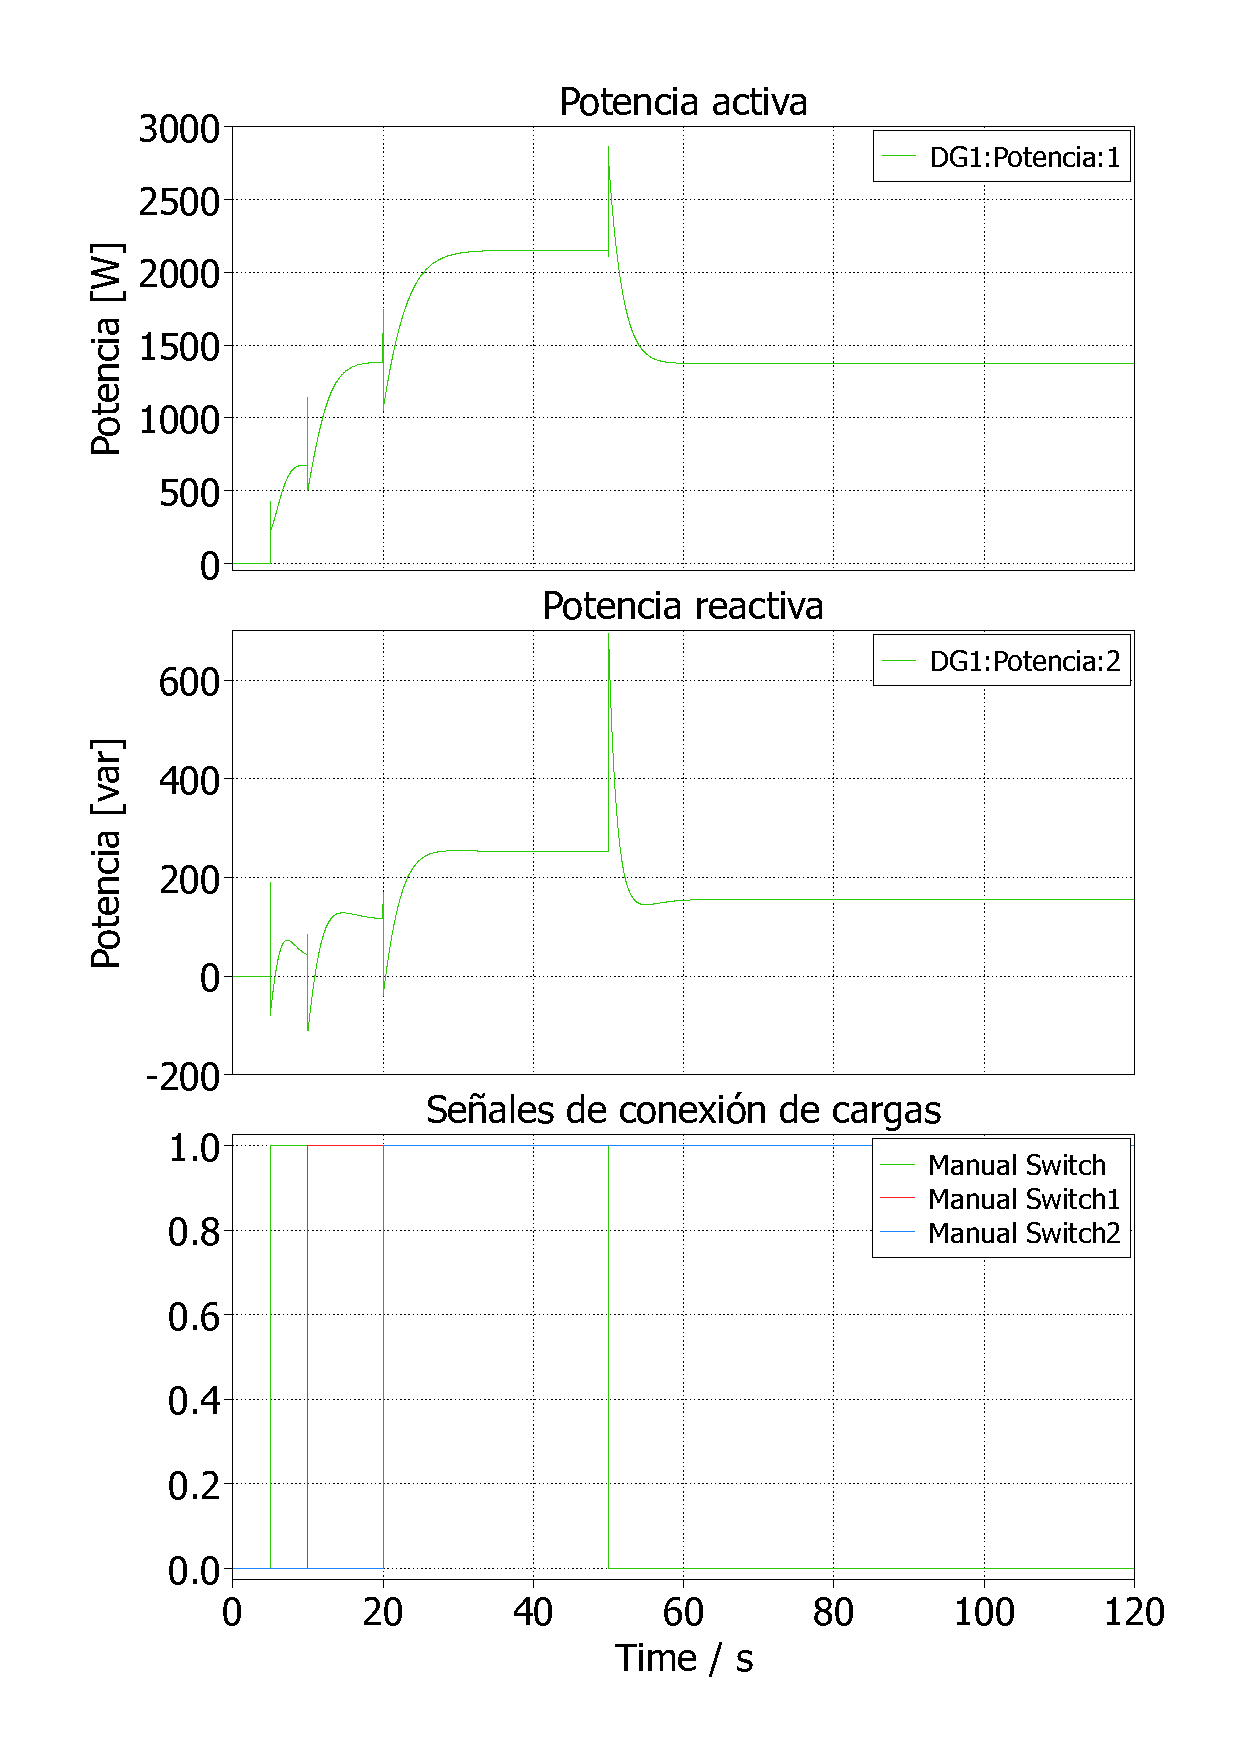
\includegraphics[width=0.5\linewidth]{Tarea 1/report/imagenes/p3a/droop_3.pdf}
   \caption{Potencia calculada con $Mp = -0.000036$ y $Mq_-0.0018$.}
   \label{droop_3}
\end{figure}
